\ifdefined\pdfinfoomitdate\pdfinfoomitdate=1\fi
\ifdefined\pdftrailerid\pdftrailerid{}\fi
\ifdefined\pdfsuppressptexinfo\pdfsuppressptexinfo=15\fi
\newcommand{\DoNotLoadEpstopdf}{}
\documentclass[11pt]{article}
\usepackage[T1]{fontenc}
\usepackage{lmodern}
\usepackage[a4paper,margin=29mm]{geometry}
\usepackage{amsmath,amssymb,amsthm,mathtools,mathrsfs}
\usepackage{microtype,enumitem,booktabs,array,graphicx,xcolor,tikz}
\usetikzlibrary{arrows.meta,positioning,calc}
\usepackage{hyperref}
\usepackage[capitalise,nameinlink,noabbrev]{cleveref}
\hypersetup{pdftitle={Deterministic Polynomial Factorization over Prime Fields},
 pdfauthor={OpenAI},colorlinks=true,linkcolor=blue!45!black,
 citecolor=blue!45!black,urlcolor=blue!45!black}
\numberwithin{equation}{section}
\newtheorem{theorem}{Theorem}[section]
\newtheorem{proposition}[theorem]{Proposition}
\newtheorem{lemma}[theorem]{Lemma}
\newtheorem{corollary}[theorem]{Corollary}
\theoremstyle{definition}
\newtheorem{definition}[theorem]{Definition}
\newtheorem{hypothesis}[theorem]{Hypothesis}
\theoremstyle{remark}
\newtheorem{remark}[theorem]{Remark}
\newcommand{\Fp}{\mathbf F_p}
\newcommand{\Fq}{\mathbf F_q}
\newcommand{\Z}{\mathbf Z}
\newcommand{\Q}{\mathbf Q}
\newcommand{\C}{\mathbf C}
\DeclareMathOperator{\Gal}{Gal}
\DeclareMathOperator{\Pic}{Pic}
\DeclareMathOperator{\Tr}{Tr}
\DeclareMathOperator{\Nm}{N}
\DeclareMathOperator{\End}{End}
\DeclareMathOperator{\Hom}{Hom}
\DeclareMathOperator{\ord}{ord}
\DeclareMathOperator{\divisor}{div}
\DeclareMathOperator{\Spec}{Spec}
\DeclareMathOperator{\im}{im}
\setlist{leftmargin=*,itemsep=3pt}
\allowdisplaybreaks[2]
\emergencystretch=2em
\title{Deterministic Polynomial Factorization over Prime Fields}
\author{OpenAI}
\date{October 4, 2026}
\begin{document}
\maketitle
\begin{abstract}
We give a uniform deterministic polynomial-time algorithm for complete
factorization over prime fields. For a prime $p$ in binary and a nonzero
polynomial $f\in\Fp[x]$ given by its dense coefficient list, the algorithm
computes the irreducible factors and their multiplicities using a number of
bit operations polynomial in $(\deg f+1)\log p$. The proof uses the uniform
Hecke zero-free theorem from the companion paper \emph{Primitive roots for
every admissible integer base}.
\end{abstract}
\tableofcontents
\section{Introduction}\label{sec:introduction}

Let $p$ be a prime, given in binary, and let $f\in\Fp[x]$ be a
nonzero polynomial, given by its dense coefficient list. Write
$n=\deg f$ and $L=\lceil\log_2 p\rceil$. Complete factorization means
computing the leading coefficient $c$ and distinct monic irreducible
polynomials $g_i$, with positive integer multiplicities $e_i$, such that
\[
 f=c\prod_i g_i^{e_i}.
\]
The empty product is permitted when $n=0$. The complexity parameter is
$(n+1)L$, so an algorithm polynomial in $p$ does not give a polynomial-time
algorithm in the prescribed representation.

Finite-field factorization is a basic constructive problem in algebra.
It also exposes a persistent distinction between randomized and
deterministic computation: a random element of a product of finite fields
often separates its components, whereas constructing a separator uniformly
can require additional arithmetic information. The present paper isolates
one form of that information and gives a deterministic splitting procedure
once it is available. To supply it uniformly, we use the zero-free theorem
for finite-order Hecke $L$-functions in the companion paper
\cite[Theorem~1.2]{OpenAIPrimitive26}. We state that input precisely in
Theorem~\ref{analytic:hecke} and prove its auxiliary-prime consequence
here. The analytic theorem itself belongs to the companion.

\begin{theorem}\label{thm:factorization}
There is a uniform deterministic algorithm that, given a prime $p$ in
binary and a nonzero dense polynomial $f\in\Fp[x]$ of degree $n$, outputs
its leading coefficient and its distinct monic irreducible factors with
their multiplicities in
\[
 O\bigl(((n+1)\lceil\log_2p\rceil)^{10^{12}}\bigr)
\]
bit operations, with absolute implied constant. A constant polynomial
returns an empty factor list. The algorithm uses no randomness,
integer-factorization oracle, primitive-root oracle, or GRH assumption.
\end{theorem}

The exponent is deliberately generous. The point is one fixed polynomial
bound for all degrees and prime characteristics. We separate the
algebraic construction from its analytic input in the following reduction.

\subsection{The auxiliary-prime reduction}

Put
\begin{equation}\label{eq:B}
 B=20+(n+1)(L+1).
\end{equation}
For a prime $q\le n$, call a rational prime $\ell$ an
\emph{auxiliary prime for $(p,q)$} if
\begin{equation}\label{eq:auxiliary}
 \ell\notin\{2,3,p,q\},\qquad \ell\equiv1\pmod{12q},\qquad
 p^{(\ell-1)/q}\not\equiv1\pmod\ell.
\end{equation}
Thus $p$ is not a $q$th power modulo $\ell$. The congruence modulo $12q$
is convenient for the analytic construction in Section~\ref{sec:analytic};
the algebraic construction only requires the corresponding congruence
modulo $q$.

\begin{theorem}\label{thm:reduction}
There is a uniform deterministic algorithm with the following guarantee.
Its input is a prime $p$ and a nonzero dense polynomial $f\in\Fp[x]$.
If $p>B^{200000}$ and $n\ge2$, its input also includes one auxiliary
prime $\ell_q$ satisfying \eqref{eq:auxiliary} for each prime $q\le n$.
It outputs the complete factorization of $f$, including multiplicities.
Let $E=\max(2,\max_q\ell_q)$, with $E=2$ when no auxiliary primes are
required. For an absolute constant $C$, the algorithm uses
$O((B+E)^C)$ bit operations. It uses neither randomness nor an integer
factorization or primitive-root oracle.
\end{theorem}

The dependence on $E$ is on the numerical value of the auxiliary primes,
not merely their bit lengths. Consequently Theorem~\ref{thm:reduction}
becomes a polynomial-time factorization theorem when these primes are
bounded by a fixed power of $B$. Upward search, trial division, and modular
exponentiation then construct them within the same kind of bound. We prove
this consequence from the cited zero-free theorem in
Section~\ref{sec:analytic}. The reduction in
Theorem~\ref{thm:reduction} does not use that theorem.

\subsection{History and the role of the construction}
\label{sec:history}

Berlekamp's algorithms put linear algebra at the center of finite-field
factorization: Frobenius-fixed elements in the quotient algebra encode its
irreducible factors, and polynomial greatest common divisors turn suitable
such elements into factors~\cite{Berlekamp67,Berlekamp70}.  Randomized
algorithms, including Cantor--Zassenhaus~\cite{CantorZassenhaus81}, obtain
expected polynomial running time by finding separating elements with random
choices.  The difficulty studied here is to make every such choice
deterministically, with a bound polynomial in both the degree and the bit
length of the characteristic.

Several deterministic results delineate this difficulty.  Shoup's algorithm
has polynomial dependence on the degree and a
$p^{1/2+o(1)}$ dependence on the characteristic~\cite{Shoup90}.
Under the generalized Riemann hypothesis, R\'onyai obtained polynomial
bounds when the number of irreducible factors is bounded~\cite{Ronyai88},
and Evdokimov obtained a bound
$(n^{\log n}\log p)^{O(1)}$ for general degree~\cite{Evdokimov94}.
The latter is quasipolynomial in $n$. The reduction proved here, combined
with the fixed-width zero-free strip that follows immediately from Hecke
GRH, already gives a polynomial bound in both parameters under GRH.
For Theorem~\ref{thm:factorization}, the companion supplies that strip
without GRH. In particular, the hypotheses and
parameters of a deterministic result matter: removing random choices
alone does not establish a uniform polynomial bound in $(n+1)L$.

Geometric methods already have an important place in this history.
Schoof's elliptic-curve method computes a square root of a fixed integer
$a$ modulo a varying prime, when one exists, in time polynomial in $\log p$; the uniform
bound in the two parameters is polynomial in $|a|$ and $\log p$, rather
than in their binary lengths~\cite[Section~4]{Schoof85}.
Pila's computation of Frobenius on abelian varieties yields deterministic
construction of roots of unity of fixed odd prime order modulo primes
congruent to $1$ modulo that order, with a running-time exponent that may
depend on the order and on the geometric
presentation~\cite[Theorems~A and~D]{Pila90}.  These results motivate
careful accounting for the varying curve and prime in the present
construction.  We must bound the degrees of field extensions, the sizes
of divisor representations, and the dimensions of all linear systems by
fixed powers of the original input parameters.

For a single prime not dividing the discriminant of an integral lift,
R\'onyai obtained, under GRH, deterministic bounds involving the degree
of that lift's splitting field~\cite{Ronyai92}.
A different kind of uniformity arises when reductions modulo many primes
are processed together.  Altman's unconditional algorithm takes
a monic irreducible polynomial in $\mathbb Z[x]$ of coefficient height
at most $H\ge2$, with splitting-field degree $m$, and factors its
reductions modulo every prime below $X$ in total time
\[
 \pi(X)(m\log H)^{O(1)}\log^5X.
\]
This is an amortized result over primes~\cite[Theorem~1.1]{Altman2025}.
The parameter $m$ can be as large as the factorial of the polynomial's
degree.  Thus this result does not give the worst-case single-input
bound sought here.  Altman's introduction also provides a recent account
of the general deterministic problem and its remaining obstacles.

The algebraic techniques used below have substantial precedents.
Computation at unknown roots by working in a quotient algebra and
splitting it when a zero test distinguishes components is an instance of
dynamic evaluation~\cite{DellaDoraDicrescenzoDuval85,Duval94}.
The digit calculations in primary multiplicative groups are the
prime-power part of the Pohlig--Hellman algorithm~\cite{PohligHellman78}.
R\'onyai already proved that a completely split polynomial of even degree
can be split in polynomial time when a quadratic nonresidue is
supplied~\cite{Ronyai88}; we include an explicit tournament proof suited
to our representation.  The odd-degree construction uses cyclic curves
$Y^q=F(X)$.  The cyclotomic action on their Jacobians and descriptions of
its first torsion layer by ramification divisors are familiar from
explicit descent, notably the work of Poonen and
Schaefer~\cite[Sections~4 and~6]{PoonenSchaefer97}.

Our effective treatment of divisors also builds on established
computational geometry.  Ideal representations on superelliptic curves,
Riemann--Roch algorithms, and finite-dimensional linear algebra for
Jacobian arithmetic appear in
\cite{GPS02,Hess02,KhuriMakdisi04}.  For norm equations, we use the
relation between cyclic algebras and norms, and the approach through
maximal orders and minimal left ideals developed in explicit
matrix-algebra computations~\cite{GilleSzamuely06,IRS12,IKR18}.
The general function-field algorithm of Ivanyos, Kutas, and R\'onyai
uses a finite-field polynomial-factorization oracle.  Here the cyclic
presentation gives explicit local orders, and evaluation of their global
sections at a rational point gives a rank-one idempotent by linear
algebra.  The structural explanation uses the splitting of vector
bundles on the projective line~\cite{Grothendieck57,HazewinkelMartin82}.

The substantive step of the present reduction is the odd-degree
separator, together with a uniform implementation of the divisor-class
divisions it requires.  A filtration of lifted ramification classes
keeps the necessary field extensions of polynomial degree.  A lattice
of divisors at infinity then forces two ramification points to receive
different labels.  We prove this mechanism and its algorithms directly;
the earlier results just discussed provide their mathematical context.
The separate step of finding sufficiently small auxiliary primes is
isolated in Section~\ref{sec:analytic}, which is the only place the
companion's analytic theorem enters.

\subsection{Proof strategy}

The Berlekamp algebra reduces complete factorization to splitting a monic
square-free polynomial $F$ all of whose roots already belong to $\Fp$.
Write $N=\deg F\ge2$. The unknown roots are represented simultaneously
by the finite algebra $\Fp[T]/(F)$; an operation whose outcomes differ
between components immediately produces a factor by a greatest common
divisor. We can therefore describe computations at an unspecified root
and carry them out without first finding that root.

The auxiliary primes construct the multiplicative information needed in
these computations. For each odd prime $q$, they give a field
$K_q=\Fp(\zeta_q)$ and a generator of the full $q$-primary subgroup of
$K_q^*$. The entry for $q=2$ is a generator of the full $2$-primary
subgroup of $\Fp^*$. Here the $q$-primary subgroup consists of the
elements whose orders are powers of $q$. These entries permit extraction
of promised $q$th roots in finite algebras by small-prime discrete
logarithms. Their construction proceeds in increasing $q$: the only
factorization needed to make the entry for $q$ has degree $q-1$.

When $N$ is even, differences between pairs of roots and the $2$-primary
entry orient the complete graph on the roots. Opposite differences have
opposite orientations. The vertex scores cannot all be equal when $N$
is even, so they provide a separator. The more substantial construction
handles odd $N$.

Choose an odd prime $q\mid N$, and write $r=v_q(N)$. Over an explicitly
constructed field $k$ of degree at most $N(q-1)$ over $\Fp$, consider
the smooth projective curve with affine equation
\[
 C:\quad Y^q=F(X).
\]
Its ramification points are $P_i=(x_i,0)$, where the $x_i$ are the
unknown roots of $F$. There are $q$ rational points at infinity.
The automorphism $\sigma(X,Y)=(X,\zeta_qY)$ acts on degree-zero divisor
classes; write $\lambda=1-\sigma$. Degree-zero divisors supported at
infinity form a lattice on which $\lambda$ is injective. In contrast,
$\lambda$ is surjective on the geometric Jacobian.

This difference is the source of the splitting argument. We lift each
class $[P_i-\infty_0]$ repeatedly through $\lambda$, keeping track of
an infinity divisor at every stage. A filtration argument shows that all
the classes required for these lifts are rational over the field $k$;
the extension degree stays polynomial even though the number of possible
classes is large. Summing the lifted classes and applying explicit label
tests forces a distinction between ramification points. If every test
gave one common label, a fixed nonzero infinity divisor would become
divisible by one more power of $\lambda$ than its lattice valuation
allows.

The geometric existence argument is accompanied by a constructive
division algorithm. A promised $\lambda$-division reduces to a norm
equation in $k(C)/k(X)$. We solve that equation by constructing maximal
orders in a split cyclic algebra and computing their global sections
on the projective line. A rank-one idempotent in this algebra yields
the norm solution. All computations use polynomial and matrix arithmetic;
Riemann--Roch reduction controls divisor sizes, and arithmetic circuits
store principal functions arising from large infinity multiplicities.
Figure~\ref{fig:route} records the roles of these ingredients.

\begin{figure}[t]
\centering
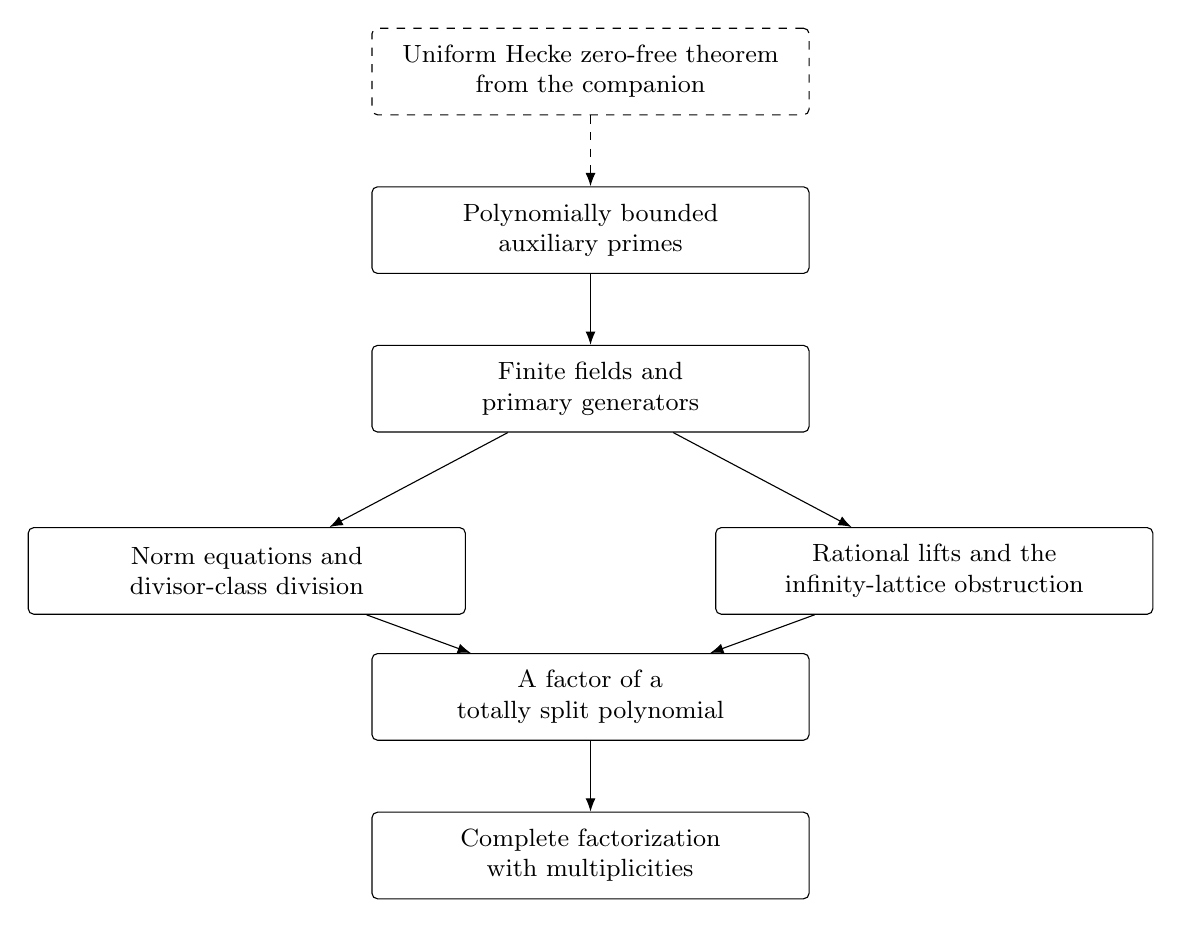
\begin{tikzpicture}[font=\small,>=Latex,
 box/.style={draw,rounded corners=2pt,align=center,text width=5.2cm,
 minimum height=11mm,inner sep=5pt},node distance=9mm and 12mm]
 \node[box,dashed] (analytic) {Uniform Hecke zero-free theorem\\from the companion};
 \node[box,below=of analytic] (primes) {Polynomially bounded auxiliary primes};
 \node[box,below=of primes] (table) {Finite fields and\\primary generators};
 \node[box,below left=12mm and -12mm of table] (norm)
   {Norm equations and\\divisor-class division};
 \node[box,below right=12mm and -12mm of table] (geometry)
   {Rational lifts and the\\infinity-lattice obstruction};
 \node[box,below=28mm of table] (split) {A factor of a\\totally split polynomial};
 \node[box,below=of split] (factor) {Complete factorization\\with multiplicities};
 \draw[->,dashed] (analytic)--(primes);
 \draw[->] (primes)--(table);
 \draw[->] (table)--(norm);
 \draw[->] (table)--(geometry);
 \draw[->] (norm)--(split);
 \draw[->] (geometry)--(split);
 \draw[->] (split)--(factor);
\end{tikzpicture}
\caption{The proof separates auxiliary-prime existence from the algebraic
reduction. The dashed implication uses the cited analytic theorem;
the remaining constructions are proved in the paper. The two middle
branches are the effective and geometric parts of the odd-degree splitter.}
\label{fig:route}
\end{figure}

The technical results are uniform in the degree of the curve and the
prime $q$. This uniformity is essential: a running-time exponent depending
on the genus would not suffice for Theorem~\ref{thm:reduction}.
We give the finite-field tools first, then the auxiliary table, the
geometry, and the effective divisor and norm calculations. The splitter
and the factorization driver assemble these ingredients. The final two
sections prove the bit bounds and the analytic implication.

\section{Finite-field computations without known roots}
\label{ff:section}

The splitting procedures will manipulate all roots of a polynomial at once.
Two elementary tools make this possible.  First, a computation over a field
can be executed in a product of fields until a zero test distinguishes two
components.  Second, a supplied generator of a primary multiplicative subgroup
permits logarithms and root extraction by short digit calculations.  We develop
both tools explicitly, and then use them to split every totally split polynomial
of even degree.

Finite fields are represented by a basis over their prime field and a
multiplication table, or by an equivalent tower of polynomial quotients.
Field arithmetic, binary powering, polynomial Euclidean algorithms, and linear
algebra are therefore deterministic procedures with polynomial bit complexity
in the representation lengths.  All basis choices and pivot choices below use
a fixed ordering.  For a prime $q$ and a positive integer $m$, write
$v_q(m)$ for its $q$-adic valuation.  If $k$ has cardinality $Q$ and
$q\mid Q-1$, its full $q$-primary subgroup is the unique subgroup of
$k^*$ of order $q^{v_q(Q-1)}$.

\subsection{Simultaneous execution and zero tests}

Let $k$ be an explicitly represented finite extension of $\mathbf F_p$, and let
$F\in\mathbf F_p[T]$ be monic, square-free, and totally split, of degree $N$.
Write its roots as $x_1,\ldots,x_N$ for the proof; the algorithm does not know
these roots.  The algebra
\begin{equation}
 A=k[T]/(F)\simeq\prod_{i=1}^N k,
 \qquad a(T)\longmapsto(a(x_1),\ldots,a(x_N))
 \label{ff:product}
\end{equation}
lets us carry out arithmetic on all components simultaneously.

\begin{lemma}[Simultaneous execution]
\label{ff:simultaneous}
Suppose a deterministic field procedure uses arithmetic, zero tests, and
integer control, and its scalar input at component $i$ is obtained by
specializing given elements of $A$ at $T=x_i$.  Assume the procedure is
defined for each specialized input.  One can either execute the
procedure on all components with a common sequence of decisions, or return a
nontrivial proper monic divisor of $F$ in $\mathbf F_p[T]$.
The extra cost of each scalar operation or zero test is polynomial in
$N$, $[k:\mathbf F_p]$, and $\log p$.
\end{lemma}

\begin{proof}
For a zero test on $a\in A$, compute $d=\gcd(F,a)$ over $k$ using its
representative of degree less than $N$.  If $d=1$, every component is nonzero;
if $d=F$, every component is zero.  In the remaining case, $d$ is a proper
factor and the procedure stops.  Although computed over $k$, its monic form
belongs to $\mathbf F_p[T]$: it is the product of $T-x_i$ over the components
where $a(x_i)=0$.

Addition and multiplication take place in $A$.  A nonzero scalar is inverted
only after the zero test has shown it nonzero in every component; the extended
Euclidean algorithm then gives its inverse modulo $F$.  Thus, until a split
occurs, every field instruction and decision is valid in every component.
Polynomial degree tests and choices of pivots reduce to successive zero tests
on coefficients, so the same argument applies inside polynomial arithmetic
and linear algebra.  The usual dense implementations give the cost bound.
\end{proof}

This is the dynamic-evaluation principle~\cite{DellaDoraDicrescenzoDuval85};
we call its use here \emph{simultaneous execution}.  In particular, a
divergent pivot or a divergent polynomial degree is useful information: it
already supplies the required factor.  The convention also applies to nested
procedures whose coefficient field is being simulated by $A$.

\subsection{Logarithms in primary subgroups}

Let $q$ be a prime, and suppose $u$ generates a cyclic group of order $q^s$.
For $a\in\langle u\rangle$, its logarithm $\ell\in[0,q^s)$ can be recovered
one base-$q$ digit at a time, as in the prime-power logarithm algorithm of
Pohlig and Hellman~\cite{PohligHellman78}.  If $\ell_j\equiv\ell\pmod{q^j}$ is already
known, the next digit is the unique $c\in\{0,\ldots,q-1\}$ satisfying
\begin{equation}
 (au^{-\ell_j})^{q^{s-j-1}}
   =(u^{q^{s-1}})^c,
 \qquad 0\le j<s.
 \label{ff:digit}
\end{equation}
Set $\ell_{j+1}=\ell_j+cq^j$ and begin with $\ell_0=0$.
Indeed, if $\ell-\ell_j=q^j(c+qv)$, raising to $q^{s-j-1}$ removes the term
$qv$ and leaves exactly Equation~\eqref{ff:digit}.  This uses $q$ equality
tests per digit, rather than an enumeration of $q^s$ group elements.

The same calculation works in a product of fields when $u$ has order $q^s$
in every component.  When the product is presented as $k[X]/H$ with $H$
square-free, gcds with $H$ partition the components at each digit according
to the equality in Equation~\eqref{ff:digit}; retain each nonempty piece and
its current digit string.  There are at most $\deg H$ pieces at every level.
Keep each final integer logarithm together with its polynomial modulus.
Algebra elements subsequently computed from these logarithms can be recombined
by polynomial Chinese remaindering.  Alternatively, when zero components are represented by idempotent masks,
perform the same partitions using those masks.  These two implementations
will be used below.

\subsection{Root extraction in a finite reduced algebra}

We next give the root procedure used in the norm equations later in the paper.
Its input already includes a generator over the constant field, but it does
not include generators in extension fields, nor a factorization of the
modulus.

\begin{lemma}[Root extraction from a primary generator]
\label{ff:unitroot}
Let $k$ be an explicit finite field of cardinality $Q$ and characteristic $p$.
Let $q$ be an odd prime dividing $Q-1$, let $\zeta\in k$ have order $q$, and
let $\omega\in k$ generate the full $q$-primary subgroup of $k^*$.
Let $H\in k[X]$ be monic and square-free, with $h=\deg H\ge1$, and suppose
$p>h^2$.  Given a unit $a\in k[X]/H$ that is promised to be a $q$-th power,
one can deterministically construct $b$ with $b^q=a$.
The bit cost is polynomial in $q$, $h$, and the length of the given field
representation.  The procedure uses only arithmetic and zero tests over $k$,
and so admits simultaneous execution as in Lemma~\ref{ff:simultaneous}.
\end{lemma}

\begin{proof}
The construction has three steps: separate extension degrees, obtain a primary
generator on each resulting part, and take the two coprime parts of the root.

\smallskip
\noindent\emph{Separate extension degrees.}
For $d=1,\ldots,h$, use gcds with $X^{Q^d}-X$, removing factors already found,
to form the product $H_d$ of the irreducible factors of $H$ of degree $d$.
All powers are computed modulo the current modulus by binary powering.
Discard $H_d=1$.  Every field component of $k[X]/H_d$ has cardinality $Q^d$.
Write
\[
 Q^d-1=q^s t,\qquad q\nmid t.
\]
Only division by the specified prime $q$ is needed to find $s$ and $t$.

\smallskip
\noindent\emph{Obtain a primary generator.}
Since $q$ is odd and $q\mid Q-1$, the elementary lifting-the-exponent identity
is
\begin{equation}
 v_q(Q^d-1)=v_q(Q-1)+v_q(d).
 \label{ff:lte}
\end{equation}
To see this, raising a number congruent to $1$ modulo $q$ to an exponent
prime to $q$ preserves the valuation of its difference from $1$, whereas
raising it to the $q$-th power increases that valuation by exactly one.
Both assertions follow from the binomial expansion: its linear term has
strictly smaller $q$-valuation than all subsequent terms, using that $q$
is odd in the second assertion.  Iterating proves Equation~\eqref{ff:lte}.
If $q\nmid d$, set $u=\omega$, which already has order $q^s$ in every
component.  Suppose instead that $q\mid d$.  Solve the $k$-linear equation
\begin{equation}
 v^{Q^{d/q}}=\zeta v
 \quad\text{in }k[X]/H_d.
 \label{ff:eigenvector}
\end{equation}
In each component its nonzero solutions exist: the cyclic group of order
$Q^d-1$ contains a solution of $v^{Q^{d/q}-1}=\zeta$, because
\[
 \zeta^{(Q^d-1)/(Q^{d/q}-1)}=1.
\]
For such a solution, Equation~\eqref{ff:lte} shows that the $q$-valuation of
its order is $s$.

To choose a solution nonzero in every component without knowing those
components, take a kernel basis $v_0,\ldots,v_{r-1}$ and try
\begin{equation}
 v(c)=\sum_{j=0}^{r-1}c^jv_j,
 \qquad c=0,\ldots,h^2.
 \label{ff:unit-search}
\end{equation}
Test each candidate for being a unit by a gcd with $H_d$.  In any component,
at least one basis vector is nonzero, so at most $r-1$ values of $c$ make
$v(c)$ zero there.  There are at most $h$ components and $r\le h$; fewer than
$h^2$ values are excluded altogether.  The hypothesis $p>h^2$ makes the
listed parameters distinct.  Hence the search succeeds.  Raising its result
to $t$ produces a generator $u$ of order $q^s$ in every component.

\smallskip
\noindent\emph{Take the root.}
Use the integer Chinese remainder theorem for $q^s$ and $t$ to choose
exponents projecting $a$ to its primary and prime-to-$q$ parts.  Explicitly,
put
\[
 a_q=a^{t(t^{-1}\bmod q^s)},\qquad
 a_t=a^{q^s((q^s)^{-1}\bmod t)},
\]
with $a_t=1$ when $t=1$.  Then $a=a_q a_t$, the order of $a_q$ divides
$q^s$, and the order of $a_t$ divides $t$.  A root of $a_t$ is obtained by
raising it to $q^{-1}\bmod t$, again using $1$ when $t=1$.

Compute the logarithm of $a_q$ to $u$ by Equation~\eqref{ff:digit},
partitioning $H_d$ as necessary.  In each final piece its logarithm
$\ell\in[0,q^s)$ is divisible by $q$, because $a$ is a $q$-th power.
Therefore $u^{\ell/q}$ is a root of $a_q$ on that piece.  Multiply the two
roots, recombine the pieces by polynomial Chinese remaindering, and finally
recombine the relatively prime $H_d$.

For complexity, $d\le h$, the bit length of $Q^d$ is at most $1+h\log_2Q$,
and $s\le h\log_2Q$.  There are at most $h$ nonempty pieces at every digit
level; each digit tests at most $q$ possibilities.  Equation~\eqref{ff:eigenvector}
is a linear system of dimension at most $h$, and
Equation~\eqref{ff:unit-search} uses at most $h^2+1$ trials.  All remaining
operations are polynomial arithmetic, powering, or integer Euclidean
algorithms of the indicated sizes.  This proves the claimed polynomial
bound and also the assertion about field instructions.
\end{proof}

We denote this procedure by $\mathsf{UnitRoot}$.  To extract a root in $k$
itself, apply it with the linear modulus $H=X$.  The proof explains why
distinct-degree decomposition suffices: every subsequent partition is obtained
by an equality test, and full irreducible factorization is never invoked.

\subsection{Splitting an even number of roots}

R\'onyai proved that a supplied quadratic nonresidue suffices to split
a completely split polynomial of even degree in polynomial time~\cite{Ronyai88}.
A quadratic nonresidue gives a full $2$-primary generator by raising it to
the odd part of $p-1$.  We give the pair-orientation argument in the form
needed here.  A primary generator forces a distinction among an even number of
roots.  The mechanism is an orientation of the pairs of distinct roots: each
pair contributes one to precisely one of its two row counts.  Equal row
counts would then have the nonintegral value $(N-1)/2$.

\begin{proposition}[Even-degree splitting]
\label{ff:even-split}
Let $p$ be odd, and let $F\in\mathbf F_p[T]$ be monic, square-free, and
totally split of even degree $N\ge2$, with $p>N$.  Given a generator $u$ of
the full $2$-primary subgroup of $\mathbf F_p^*$, one can deterministically
find a nontrivial proper monic divisor of $F$ in a number of bit operations
polynomial in $N$ and $\log p$.
\end{proposition}

\begin{proof}
Set $A=\mathbf F_p[T]/F$ and $R=A\otimes_{\mathbf F_p}A$.  Write
$p-1=2^s t$ with $t$ odd.  In the coordinate description indexed by ordered
pairs of roots, the element
\[
 \Delta=T\otimes1-1\otimes T
\]
has coordinate $x_i-x_j$.  Thus $e=\Delta^{p-1}$ is the idempotent equal to
$1$ off the diagonal and $0$ on the diagonal.  Work in the algebra $eR$,
whose identity is $e$.  The element $\Delta^t$ has $2$-power order at every
coordinate there, so compute its logarithm to $u$ by the digit procedure.
For a masked equality test on an element $z$ in a subalgebra with identity
mask $e_0$, its zero mask is $e_0-(e_0z)^{p-1}$.  Hence every partition is
computed within $R$, with no knowledge of the roots.

Let $e_*$ be the sum of the final masks whose logarithms lie in
$[0,2^{s-1})$.  Replacing $(i,j)$ by $(j,i)$ changes $\Delta^t$ to its
negative, because $t$ is odd.  The logarithm therefore changes by
$2^{s-1}$ modulo $2^s$, and exactly one orientation of each unordered pair
is selected by $e_*$.  Apply the ordinary algebra trace on the second factor:
\begin{equation}
 c=(\operatorname{id}\otimes\operatorname{Tr}_{A/\mathbf F_p})(e_*)\in A.
 \label{ff:row-counts}
\end{equation}
Its $i$-th coordinate is the number $c_i$ of selected pairs in row $i$,
viewed in $\mathbf F_p$.  As integers,
\[
 0\le c_i\le N-1,
 \qquad \sum_{i=1}^N c_i=\frac{N(N-1)}2.
\]
If these integers were all equal, their common value would be $(N-1)/2$,
which is impossible for even $N$.  Since $p>N$, their images in the field
are not all equal either.  Testing $\gcd(F,c-a)$ for $a=0,\ldots,N-1$
therefore returns a nontrivial proper factor.

The algebra $R$ has dimension $N^2$, and the number of nonempty masks at a
digit level is at most $N^2$.  There are $s\le\log_2p$ levels, each with
two possible digits.  Binary powering, the trace computation, and the final
gcds all have the asserted polynomial cost.
\end{proof}

\section{Auxiliary primes and primary generators}
\label{sec:table}

The splitting procedure needs explicit generators of small-prime parts of
multiplicative groups.  This section constructs those generators from the
auxiliary primes supplied in Theorem~\ref{thm:reduction}.
The construction uses linear algebra
in cyclotomic algebras and calls the factorization procedure only in strictly
smaller degrees.  Existence of small auxiliary primes is a separate
number-theoretic question; no size bound for them is assumed in this section.

We use the notation $v_q(a)$ and the full $q$-primary subgroup
introduced in Section~\ref{ff:section}.

Throughout the construction, $p>n\ge2$.  For each prime $q\le n$,
recall that the supplied auxiliary prime $\ell_q$ satisfies
\begin{equation}\label{table:primes}
 \ell_q\notin\{2,3,p,q\},\qquad
 \ell_q\equiv1\pmod{12q},\qquad
 p^{(\ell_q-1)/q}\not\equiv1\pmod{\ell_q}.
\end{equation}
Recall the bound $E=\max(2,\max_{q\le n}\ell_q)$ from
Theorem~\ref{thm:reduction}.  Supplied primes can be checked by trial
division and modular exponentiation in time polynomial in $E$, $n$, and
$\log p$.  The same tests can search upward for the first suitable prime;
if one exists below $E$, that search also takes time polynomial in these
parameters.  Factoring $\ell_q-1$ is unnecessary.

The table has the following contents:
\begin{itemize}
\item for $q=2$, an element $\omega_2\in\mathbb F_p^*$ of order
      $2^{v_2(p-1)}$;
\item for each odd prime $q\le n$, an explicitly represented field
      $K_q/\mathbb F_p$, an element $\zeta_q\in K_q$ of order $q$ with
      $K_q=\mathbb F_p(\zeta_q)$, and an element $\omega_q\in K_q^*$
      of order $q^{v_q(|K_q|-1)}$.
\end{itemize}
An explicit field here consists of an $\mathbb F_p$-basis, its
multiplication constants, and the coordinates of its identity.  A quotient
by a specified irreducible polynomial is an equivalent representation.
Both descriptions support arithmetic and linear algebra in polynomial time.
We use the standard structure theory of finite fields; see
\cite{LidlNiederreiter97}.

\subsection{A degree-\texorpdfstring{$q$}{q} field without factoring a cyclotomic polynomial}

Fix $q$ and $\ell=\ell_q$.  Put
\[
 R_\ell=\mathbb F_p[T]/(1+T+\cdots+T^{\ell-1}),\qquad
 \Gamma_\ell=(\mathbb Z/\ell\mathbb Z)^*,\qquad
 H_q=\{a^q:a\in\Gamma_\ell\}.
\]
For $a\in\Gamma_\ell$, let $\tau_a$ be the automorphism of
$R_\ell$ defined by substitution $T\mapsto T^a$.  Enumerate $H_q$ by taking $q$th powers modulo $\ell$,
and compute
\begin{equation}\label{table:invariants}
 U_q=R_\ell^{H_q}
    =\bigcap_{a\in H_q}\ker(\tau_a-\mathrm{id})
\end{equation}
by $\mathbb F_p$-linear algebra.  Products of basis
elements of this space, reduced in $R_\ell$ and expressed in its computed
basis, give the multiplication constants of $U_q$.

\begin{lemma}\label{table:degreeq}
The algebra $U_q$ is a field of degree $q$ over $\mathbb F_p$.
\end{lemma}
\begin{proof}
Since $p\ne\ell$, the polynomial defining $R_\ell$ has $\ell-1$
distinct roots over an algebraic closure $\overline{\mathbb F}_p$.
They are precisely the primitive $\ell$th roots of unity.  Evaluation at
these roots identifies the scalar extension of $R_\ell$ with the algebra
of functions on that set.  The group $\Gamma_\ell$ acts regularly on the
set, and its subgroup $H_q$ has index $q$.  Taking kernels commutes with
extension of scalars.  Consequently
\[
 U_q\otimes_{\mathbb F_p}\overline{\mathbb F}_p
       \simeq\overline{\mathbb F}_p^{\,q},
\]
with the factors indexed by the $H_q$-orbits.

Frobenius permutes the primitive roots by raising them to the $p$th
power, hence acts on the orbit set by multiplication by the class of $p$
in $\Gamma_\ell/H_q$.  A cyclic group of order $\ell-1$ has
$H_q=\{a:a^{(\ell-1)/q}=1\}$, so the last condition in
\eqref{table:primes} says that this class is nonidentity.  The quotient has
prime order $q$; its nonidentity elements act transitively on it.
A finite reduced algebra over a finite field is a product of finite fields,
and its field factors correspond exactly to Frobenius orbits on its
geometric points.  There is one such orbit, of length $q$, proving the
claim.
\end{proof}

This construction is useful precisely because the computation of
$U_q$ never asks for the individual irreducible factors of the degree
$\ell-1$ cyclotomic polynomial.  Its field property follows from the
verified power-residue test on the integer prime $\ell$.

\subsection{Extracting the primary generators}

For $q=2$, solve the $\mathbb F_p$-linear equation
\[
 v^p=-v\qquad(v\in U_2)
\]
and take a nonzero solution.  The trace map $v\mapsto v+v^p$ from the
quadratic field $U_2$ to $\mathbb F_p$ is nonzero, because it sends $1$
to $2$.  Its kernel has dimension one, so this instruction succeeds.
Then $c=v^2$ lies in $\mathbb F_p^*$ and
\[
 c^{(p-1)/2}=v^{p-1}=-1.
\]
Thus $c$ is a nonsquare.  With $s=v_2(p-1)$, set
\begin{equation}\label{table:quadratic}
 \omega_2=c^{(p-1)/2^s}.
\end{equation}
The order of a nonsquare in a cyclic group of even order has the full
$2$-part of that order.  The odd exponent in \eqref{table:quadratic}
therefore leaves $\omega_2$ of exact order $2^s$.

For odd $q$, first factor
\[
 \Phi_q(Z)=1+Z+\cdots+Z^{q-1}
\]
over $\mathbb F_p$.  The smaller-degree nature of this call will be
justified below.  Choose the first monic irreducible factor in a fixed
coefficient order, form its quotient field $K_q$, and let $\zeta_q$ be the
image of $Z$.  Every root of $\Phi_q$ has order $q$, because $p\ne q$.
Writing $d_q=[K_q:\mathbb F_p]$, finite-field theory gives
\[
 d_q=\operatorname{ord}_q(p)\mid q-1,
\]
where $\operatorname{ord}_q(p)$ is the multiplicative order of $p$
modulo $q$.  In particular $\gcd(d_q,q)=1$.  The tensor product
\[
 V_q=U_q\otimes_{\mathbb F_p}K_q
\]
is therefore a field of degree $q$ over $K_q$: finite fields of coprime
degrees intersect in $\mathbb F_p$, so they are linearly disjoint.
Its multiplication table is obtained directly from those of its two
factors.

Set $Q_q=|K_q|$ and $s_q=v_q(Q_q-1)$.  Solve the $K_q$-linear system
\begin{equation}\label{table:eigenvector}
 u^{Q_q}=\zeta_q u\qquad(u\in V_q)
\end{equation}
and choose a nonzero solution.  To prove existence, the homomorphism
$x\mapsto x^{Q_q-1}$ on $V_q^*$ has image equal to the norm-one subgroup
for $V_q/K_q$.  Indeed both subgroups have order
$(Q_q^q-1)/(Q_q-1)$.  The norm of $\zeta_q$ equals
$\zeta_q^{1+Q_q+\cdots+Q_q^{q-1}}=\zeta_q^q=1$.
Thus $\zeta_q$ lies in this image, proving that
\eqref{table:eigenvector} has a nonzero solution.

For odd $q$ and $Q_q\equiv1\pmod q$, the lifting-the-exponent identity is
\begin{equation}\label{table:lte}
 v_q(Q_q^a-1)=s_q+v_q(a)\qquad(a\ge1).
\end{equation}
This is Equation~\eqref{ff:lte}.  In particular $v_q(Q_q^q-1)=s_q+1$.  Equation
\eqref{table:eigenvector} says that $u^{Q_q-1}$ has order exactly $q$,
so the $q$-part of the order of $u$ is exactly $q^{s_q+1}$.  Consequently
\[
 w=u^{(Q_q^q-1)/q^{s_q+1}},\qquad \omega_q=w^q
\]
have orders $q^{s_q+1}$ and $q^{s_q}$, respectively.  The unique
subgroup of $V_q^*$ of order $q^{s_q}$ lies in $K_q^*$, since
$q^{s_q}\mid Q_q-1$.  Therefore $\omega_q\in K_q$, as required.
Its coordinates in $K_q$ are obtained by solving the linear equations for
the known inclusion $K_q\hookrightarrow V_q$.

All integer valuations used here are found by repeated division by the
specified prime $q$.  All powers use binary exponentiation.  Neither
construction requires an integer factorization of $p-1$ or $Q_q-1$.

\subsection{The increasing-degree construction}

The only call above to an as yet unspecified factoring procedure is the
factorization of $\Phi_q$, whose degree is $q-1$.  The interface with the
rest of the paper is the following.

\begin{proposition}[Table construction]\label{table:construction}
Suppose the auxiliary primes \eqref{table:primes} are supplied, and
suppose a deterministic procedure has the following uniform contract:
for every integer $1\le b<n$, it factors every monic polynomial of degree at
most $b$ over $\mathbb F_p$ using table entries only for primes at most
$b$.  Then the complete table through $n$ can be built in increasing
prime order.  Its construction calls that procedure at most once for each
odd prime $q\le n$, on a polynomial of degree $q-1$; each such call uses
only already constructed table entries.

Apart from these factorization calls, the construction has bit cost
polynomial in $E$, $n$, and $\log p$, with an absolute exponent.  Each
stored odd-prime field has degree at most $q-1$, and the temporary field
$V_q$ has degree at most $q(q-1)$ over $\mathbb F_p$.
\end{proposition}
\begin{proof}
Begin with the quadratic construction, which needs no factorization call.
For an odd prime $q$, every prime at most $q-1$ is smaller than $q$, so
the indicated factorization call has all its required entries.  Its output
constructs $K_q$, and the preceding linear-algebra construction supplies
$\omega_q$.  This proves the inductive assertion and the degree bounds.

For completeness, the largest auxiliary algebra $R_{\ell_q}$ has
dimension $\ell_q-1\le E$.  Substitution operators are computed by
modular polynomial powering.  There are at most $\ell_q-1$ elements in
$H_q$, and their fixed-space equations have at most $\ell_q-1$
unknowns.  Gaussian elimination gives its invariant subspace and its
multiplication constants in polynomial time.  All subsequent field
dimensions are at most $n^2$.  Including the modular residue tests, the exponent integers used have
$O(\log(E+1)+n^2\log p)$ bits, and each extraction of a specified prime valuation
has polynomial cost.  Schoolbook arithmetic consequently gives, for
example, an upper bound
\[
 O\bigl(n(E+1)^{10}(n+\lceil\log_2p\rceil+1)^{40}\bigr)
\]
for the work outside the factorization calls.  The same generous bound
includes trial division and upward searches through $E$.
\end{proof}

Section~\ref{driver:section} proves that \textsc{Factor} has exactly this
interface.  Its correctness and the table construction are established
by a common induction: the entry for $q$ invokes factorization only below
$q$, whereas factorization in degree $b$ invokes entries only at most
$b$.  Thus the table uses no factorization oracle.  The only external
data in this construction are the verified auxiliary primes.

\section{Divisions on a cyclic cover}
\label{geom:section}

The odd-degree splitting procedure will repeatedly divide divisor classes by
$1-\sigma$, where $\sigma$ is a cyclic automorphism of a curve.
Its first requirement is an existence statement:
all the needed divisions must be rational over an extension of polynomial
degree.  Its second requirement is a test that eventually distinguishes two
ramification points.  We establish the geometric inputs here.
The essential device is
to retain a divisor supported at infinity together with a chosen division
of its class in the Jacobian.  Equality of classes may lose information about that divisor;
retaining the divisor makes a final divisibility obstruction visible.

\subsection{The curve and its infinity lattice}
\label{geom:setup}

Let $K$ be a finite field of characteristic $p$, let $q\ne p$ be an odd
prime, and suppose that $K$ contains a primitive $q$-th root of unity $\zeta$.
Let $F\in K[X]$ be monic and square-free, of degree $N\ge q$ divisible by $q$,
and suppose that all its roots $x_1,\ldots,x_N$ belong to $K$.
Consider the smooth projective curve $C/K$ with function field
\[
                  K(C)=K(X,Y),\qquad Y^q=F(X).
\]
The roots $x_i$ serve only as mathematical indices here; their values need
not be known to an algorithm.

A simple root of $F$ has valuation one, so $F$ is not a $q$-th power even
over $\overline K(X)$.  Thus $C$ is geometrically integral and the map
$X:C\longrightarrow\mathbb P^1$ has degree $q$.  The affine equation is
smooth: a singularity would have $Y=0$ and $F(X)=F'(X)=0$.
At infinity, put
\[
 z=X^{-1},\qquad U=Yz^{N/q},\qquad
 U^q=z^N F(z^{-1}).
\]
At $z=0$ the right side is $1$, and its $q$ roots are simple.
There are therefore exactly $q$ rational points at infinity,
\[
 I=\{\infty_j:0\le j<q\},\qquad U(\infty_j)=\zeta^j.
\]
The ramification points are $P_i=(x_i,0)$.  Each is totally and tamely
ramified, and there is no other ramification.  The tame Riemann--Hurwitz
formula~\cite[Tags 0C1B and 0C1F]{StacksProject} consequently gives
\begin{equation}
                  g(C)=\frac{(q-1)(N-2)}2.
\label{geom:genus}
\end{equation}

Let $\sigma$ send $(X,Y)$ to $(X,\zeta Y)$ on points.
We let it act on functions by
\begin{equation}
                 (\sigma h)(X,Y)=h(X,\zeta^{-1}Y),
\label{geom:function-action}
\end{equation}
so that $\operatorname{div}(\sigma h)=\sigma\operatorname{div}(h)$.
In particular, $\sigma P_i=P_i$ and
$\sigma\infty_j=\infty_{j+1}$, with subscripts taken modulo $q$.

Write $J=\operatorname{Pic}^0(C_{\overline K})$ for the group of
geometric degree-zero divisor classes, and put
\[
 \Lambda=\left\{\sum_{j=0}^{q-1}a_j\infty_j:
                  a_j\in\mathbb Z,\ \sum_j a_j=0\right\}.
\]
For a degree-zero divisor $D$, its class is denoted by $[D]$.
The orbit sum $1+\sigma+\cdots+\sigma^{q-1}$ acts as zero on both $J$
and $\Lambda$.  For $J$, this follows because the orbit sum of a divisor
is the pullback of its pushforward to $\mathbb P^1$, and a degree-zero
divisor on $\mathbb P^1$ is principal.  For $\Lambda$, it follows by
summing its coefficients.

Let $R=\mathbb Z[\xi]$, where $\xi$ is an abstract primitive $q$-th root
of unity, and let $\xi$ act as $\sigma$.  The preceding orbit-sum identity
makes $J$ and $\Lambda$ into $R$-modules.  Set
\begin{equation}
             \lambda=1-\xi,\qquad e=(\sigma-1)\infty_0.
\label{geom:lambda}
\end{equation}
The differences $\sigma^j e$ generate $\Lambda$.  The resulting map
$R\longrightarrow\Lambda$, $a\longmapsto ae$, is an isomorphism:
it is surjective between free abelian groups of the same rank $q-1$.
In particular, multiplication by $\lambda$ is injective on $\Lambda$.
On divisors and divisor classes, multiplication by $\lambda$ means
$1-\sigma$.

We shall use
\begin{equation}
          q=u\lambda^{q-1}\quad\text{for some }u\in R^*,
          \qquad R/(\lambda)=\mathbb F_q.
\label{geom:cyclotomic}
\end{equation}
Indeed, $q=\prod_{a=1}^{q-1}(1-\xi^a)$, and each quotient
$(1-\xi^a)/(1-\xi)$ is an algebraic integer of norm one, hence a unit.
The quotient-ring assertion follows by setting $\xi=1$ in the
cyclotomic polynomial $1+T+\cdots+T^{q-1}$.
Multiplication by $\lambda$ is surjective on $J$.
To see this, identify $J$ with the geometric points of the Jacobian of
$C$~\cite[Theorem 1.1]{MilneJV86}.  Multiplication by $q$, which is prime
to the characteristic, is a surjective
isogeny~\cite[Theorem 8.2]{MilneAV86}.
Equation~\eqref{geom:cyclotomic} then implies the
surjectivity of multiplication by $\lambda$.

\subsection{Recording a class together with an infinity divisor}

Ramification divisors and the deck-transformation operator $1-\sigma$
also underlie explicit
descent on Jacobians of cyclic covers; see
Poonen and Schaefer~\cite[Section 6, Proposition 6.2]{PoonenSchaefer97}.
Here we record the infinity divisor as an additional coordinate, so that
successive divisions retain its integral divisibility information.

For $t\ge1$, define the $R$-module
\begin{equation}
 T_t=
 \frac{\{(d,W)\in J\times\Lambda:\lambda^t d=[W]\}}
      {\{([W'],\lambda^t W'):W'\in\Lambda\}}.
\label{geom:T-definition}
\end{equation}
A pair in the numerator will also denote its image in the quotient when
there is no ambiguity.  The quotient identifies changes obtained by adding
an infinity divisor to a representative of $d$.  Keeping $W$ itself,
instead of only its class, will allow us to test divisibility in the free
module $\Lambda$.

\begin{lemma}
\label{geom:filtration}
The module $T_t$ is killed by $\lambda^t$.  The map
\[
             T_t\longrightarrow T_{t+1},\qquad
             (d,W)\longmapsto(d,\lambda W)
\]
is injective, and its image is $T_{t+1}[\lambda^t]$.
Consequently, inside any $T_m$ the successive modules are precisely
$T_j=T_m[\lambda^j]$ for $1\le j\le m$.
\end{lemma}

\begin{proof}
For a qualifying pair, multiplication by $\lambda^t$ gives
$([W],\lambda^t W)$, which is one of the quotient relations.
The displayed map respects both the qualifying equation and the relations.
If its value is zero, then
\[
             (d,\lambda W)=([W'],\lambda^{t+1}W')
\]
for some $W'\in\Lambda$.  Injectivity of $\lambda$ on the lattice gives
$W=\lambda^tW'$, so the original pair was already zero in $T_t$.
Conversely, suppose that the class of $(d,W)$ in $T_{t+1}$ is killed by
$\lambda^t$.  There is then a $W'\in\Lambda$ such that
\[
       \lambda^t d=[W'],\qquad
       \lambda^t W=\lambda^{t+1}W'.
\]
The second equation gives $W=\lambda W'$, and $(d,W)$ is the image of
$(d,W')\in T_t$.  Iteration proves the last assertion.
\end{proof}

The first module has an explicit description in terms of the ramification
points.  This description will serve twice: it controls Frobenius on all
higher modules, and it provides the labels used to distinguish roots.

\begin{lemma}[Ramification generators and labels]
\label{geom:ramification}
In the setup of Section~\ref{geom:setup}, the elements
\[
                   \epsilon_i=([P_i-\infty_0],e)
                   \quad(1\le i\le N)
\]
generate $T_1$ over $\mathbb F_q$, and
\begin{equation}
                         \sum_{i=1}^N\epsilon_i=0.
\label{geom:sum-epsilon}
\end{equation}
More explicitly, let $D$ be a geometric degree-zero divisor, let
$W\in\Lambda$, and suppose that
\[
                  \operatorname{div}(h)=(1-\sigma)D-W.
\]
Then $\operatorname{Norm}_{\overline K(C)/\overline K(X)}(h)$ is a
nonzero constant.  Choose $\gamma\in\overline K^*$ with
\[
 \gamma^q=\operatorname{Norm}_{\overline K(C)/\overline K(X)}(h).
\]
Then $h(P_i)$ is defined and nonzero, and the residues
\begin{equation}
 l_i=v_{P_i}(D)-\log_\zeta\bigl(h(P_i)/\gamma\bigr)
                   \quad\text{in }\mathbb F_q
\label{geom:labels}
\end{equation}
satisfy
\begin{equation}
                         ([D],W)=\sum_{i=1}^N l_i\epsilon_i
                         \quad\text{in }T_1.
\label{geom:label-expansion}
\end{equation}
Here $v_{P_i}(D)$ is the coefficient of $P_i$ in $D$, and
$\log_\zeta$ is the unique exponent modulo $q$ of a $q$-th root of unity.
\end{lemma}

\begin{proof}
Since $\lambda[P_i-\infty_0]=[e]$, each $\epsilon_i$ qualifies.
The divisor of $Y$ is
\[
                 \operatorname{div}(Y)=\sum_iP_i-
                                      \frac Nq\sum_j\infty_j.
\]
Thus, with
\[
                   W'=\frac Nq\sum_j\infty_j-N\infty_0,
\]
we have $\sum_i[P_i-\infty_0]=[W']$ and $\lambda W'=Ne$.
This is exactly the relation proving~\eqref{geom:sum-epsilon}.

Now take any pair $([D],W)$ in the numerator defining $T_1$, and choose
$h$ with the stated divisor.  The orbit sum of $(1-\sigma)D-W$ is zero,
so the norm of $h$ has zero divisor on $\mathbb P^1$ and is a nonzero
constant.  Hilbert's Theorem~90~\cite[Example 2.3.4]{GilleSzamuely06}
for the cyclic extension
$\overline K(C)/\overline K(X)$ gives
\begin{equation}
                          h/\gamma=b/(\sigma b)
\label{geom:hilbert90}
\end{equation}
for some $b\in\overline K(C)^*$.
Choose an integral divisor $W_0$ supported on $I$ such that
$(1-\sigma)W_0=W$.  Such a divisor exists because the image of
$1-\sigma$ on the full permutation lattice $\mathbb Z^I$ is its
augmentation lattice $\Lambda$.  It need not have degree zero.
Taking divisors in~\eqref{geom:hilbert90} shows that
\[
                      D-\operatorname{div}(b)-W_0
\]
is invariant under $\sigma$.

An invariant divisor has equal coefficients along each unramified orbit.
At a ramification point its coefficient may be reduced modulo $q$, because
pullback multiplies that coefficient by $q$.  Hence
\begin{equation}
           D-\operatorname{div}(b)-W_0
                =\sum_i a_iP_i+X^*D_0,
          \qquad 0\le a_i<q,
\label{geom:invariant-divisor}
\end{equation}
for a divisor $D_0$ on $\mathbb P^1_{\overline K}$.
Put
\[
       W'=W_0+\Bigl(\sum_i a_i\Bigr)\infty_0
                       +(\deg D_0)\sum_j\infty_j.
\]
Taking degrees in~\eqref{geom:invariant-divisor} gives $\deg W'=0$.
A divisor of degree $\deg D_0$ on $\mathbb P^1$ is linearly equivalent
to $(\deg D_0)\infty$, so
\[
       [D]=[W']+\sum_i a_i[P_i-\infty_0],\qquad
       \lambda W'=W-\sum_i a_i e.
\]
The pair $([W'],\lambda W')$ vanishes in $T_1$, proving generation
and the expansion with coefficients $a_i$ modulo $q$.

It remains to identify these coefficients from $D$ and $h$.
At $P_i$, both $(1-\sigma)D$ and $W$ have coefficient zero.
Thus $h$ is a unit there.  Since $\sigma$ fixes $P_i$, evaluation of the
norm gives
\[
                          h(P_i)^q=\operatorname{Norm}(h).
\]
In particular $h(P_i)/\gamma$ is a power of $\zeta$.
The function $Y$ is a local parameter at $P_i$.  If
$v_{P_i}(b)=a$, the action~\eqref{geom:function-action} gives
\[
                         \bigl(b/(\sigma b)\bigr)(P_i)=\zeta^a.
\]
On the other hand, taking the coefficient of $P_i$
in~\eqref{geom:invariant-divisor} gives
$a_i\equiv v_{P_i}(D)-a\pmod q$.
Equation~\eqref{geom:hilbert90} now yields~\eqref{geom:labels} and
\eqref{geom:label-expansion}.
\end{proof}

In particular, if all the labels in~\eqref{geom:labels} agree, then
$([D],W)=0$ in $T_1$.  This implication does not require the labels to
be unique.  Replacing $\gamma$ by another $q$-th root shifts all of them
by the same constant, which has no effect because of
\eqref{geom:sum-epsilon}.

\subsection{Frobenius and rational divisions}

Let $\Pi$ denote the $|K|$-power Frobenius acting on geometric points,
divisors, and divisor classes.  It commutes with $\sigma$ and fixes
$\Lambda$ pointwise.  Lemma~\ref{geom:ramification} shows that it also
fixes $T_1$ pointwise, since all $P_i$ and all infinity points are
$K$-rational.  We next propagate this information through the filtration.

\begin{lemma}
\label{geom:frobenius}
For the curve and modules above, let $r\ge0$, set
$m=1+(q-1)r$, and let $k/K$ be the extension of degree $q^r$.
Then $\Pi^{q^r}$ fixes $T_m$ pointwise.  If $1\le t\le m$ and
$d\in J$, $W\in\Lambda$ satisfy $\lambda^t d=[W]$, then $d$ itself
is fixed by the Frobenius of $k$.
\end{lemma}

\begin{proof}
On $T_m$, let $F_j=\ker(\lambda^j)$ for $0\le j\le m$, and put
$F_j=0$ for negative $j$.  By Lemma~\ref{geom:filtration}, $F_1=T_1$.
For $1\le j\le m$ and $v\in F_j$,
\[
           \lambda^{j-1}(\Pi-1)v
                       =(\Pi-1)\lambda^{j-1}v=0.
\]
Thus $\Pi-1$ lowers the filtration by one.
Multiplication by $q$ lowers it by $q-1$, by
\eqref{geom:cyclotomic}.

Suppose that an endomorphism $A=\Pi^{q^a}-1$ lowers the filtration by
at least $f\ge1$.  The binomial expansion gives
\[
          \Pi^{q^{a+1}}-1
             =qA+\binom q2 A^2+\cdots+
                       \binom q{q-1}A^{q-1}+A^q.
\]
Every intermediate coefficient is divisible by $q$.
Its term therefore lowers by at least $f+q-1$; the last term lowers by
$qf\ge f+q-1$.  Induction shows that $\Pi^{q^r}-1$ lowers by
$1+r(q-1)=m$ and hence vanishes on $T_m$.

For the final assertion, $T_t$ embeds in $T_m$, so the class of $(d,W)$
in $T_t$ is fixed.  The lattice component is unchanged.  Consequently,
for some $W'\in\Lambda$,
\[
             (\Pi^{q^r}d-d,0)=([W'],\lambda^tW').
\]
The second coordinate and injectivity of $\lambda$ on $\Lambda$ force
$W'=0$.  The first coordinate then says $\Pi^{q^r}d=d$.
\end{proof}

For computation we need divisors and functions over $k$, not just fixed
geometric classes.  The following finite-field descent fact supplies them.
We include its proof to make the distinction explicit.

\begin{lemma}[Finite-field descent]
\label{geom:descent}
Let $C$ be a smooth projective geometrically integral curve over a finite
field $k$.  A $k$-rational divisor that is geometrically principal is the
divisor of a function in $k(C)^*$.  Every geometric divisor class fixed by
the Frobenius of $k$ has a $k$-rational divisor representative.
\end{lemma}

\begin{proof}
For the first assertion, choose a function $h$ with the given divisor over
a finite constant extension $k'/k$.  If $\tau$ generates
$\operatorname{Gal}(k'/k)$, then $\tau h/h$ is a constant in $(k')^*$,
and its norm to $k$ is one.  Hilbert's Theorem~90 for $k'/k$ lets us
scale $h$ by a constant so that it is fixed by $\tau$.

For the second assertion, choose a representative $D$ over some finite
extension $k'/k$.  Since its class is fixed,
$D-\tau D$ is principal.  The first assertion, applied over $k'$,
supplies $h\in k'(C)^*$ with
\[
                         D-\tau D=\operatorname{div}(h).
\]
The norm of $h$ in the constant-field extension has zero divisor, hence
is a constant in $k^*$.  The norm $(k')^*\to k^*$ is surjective, so a
constant multiple of $h$ has norm one.  Hilbert's Theorem~90 for
$k'(C)/k(C)$ now gives $h=b/(\tau b)$ after that scaling.
It follows that $D-\operatorname{div}(b)$ is invariant under $\tau$.
An invariant divisor descends by grouping its points into Galois orbits,
and its class is the class of $D$.
\end{proof}

\begin{corollary}
\label{geom:lifts}
In the setup of Section~\ref{geom:setup}, let $r\ge0$,
$m=1+(q-1)r$, and $[k:K]=q^r$.
For every $i$ there exist classes $d_{i,1},\ldots,d_{i,m}$, all represented
by degree-zero divisors over $k$, such that
\begin{equation}
 \begin{split}
 d_{i,1}&=[P_i-\infty_0],\\
 \lambda d_{i,t+1}&=d_{i,t}\quad(1\le t<m),\\
 \lambda^t d_{i,t}&=[e]\quad(1\le t\le m).
 \end{split}
\label{geom:lift-chain}
\end{equation}
Moreover, every successive choice of a geometric division in such a chain
has a representative over $k$.
\end{corollary}

\begin{proof}
Surjectivity of $\lambda$ on $J$ permits each successive choice over
$\overline K$.  The identity $\lambda d_{i,1}=[e]$ and induction give
the last equation in~\eqref{geom:lift-chain}.
Thus $(d_{i,t},e)$ qualifies for $T_t$.
Lemma~\ref{geom:frobenius} fixes $d_{i,t}$ over $k$, and
Lemma~\ref{geom:descent} supplies its divisor representative over $k$.
The argument applies to every chosen division, not merely to a special
compatible family.
\end{proof}

\subsection{Why the labels must separate ramification points}

Set $r=v_q(N)$ in Corollary~\ref{geom:lifts} and sum the last members of
its lift families.  The resulting class $d_m=\sum_i d_{i,m}$ satisfies
$\lambda^m d_m=[Ne]$.  This single relation is enough to force a
distinction between ramification points; the particular choices of lifts
no longer matter.  We now prove that assertion before turning to the
algorithms that construct the divisors and evaluate their labels.

\begin{proposition}[Forced separation]
\label{geom:separation}
In the setup of Section~\ref{geom:setup}, put $r=v_q(N)$ and
$m=1+(q-1)r$, and let $k/K$ have degree $q^r$.
Let $d_m\in J$ have a degree-zero divisor representative over $k$ and
satisfy $\lambda^m d_m=[Ne]$.
For $1\le t\le m$, set
\begin{equation}
           d_t=\lambda^{m-t}d_m,\qquad
           W_t=\lambda^{-(t-1)}Ne\in\Lambda,
\label{geom:separation-data}
\end{equation}
and choose any degree-zero divisor $D_t$ over $k$ representing $d_t$.
The lattice divisions defining $W_t$ exist and are unique.

Starting at $t=1$, make the following test, advancing to $t+1$ only when
all labels at $t$ agree.  Choose $h_t\in k(C)^*$ and $\gamma_t\in k^*$
such that
\begin{equation}
 \operatorname{div}(h_t)=(1-\sigma)D_t-W_t,
       \qquad \gamma_t^q=\operatorname{Norm}(h_t),
\label{geom:separation-functions}
\end{equation}
and form the labels
\begin{equation}
            l_{i,t}=v_{P_i}(D_t)
               -\log_\zeta\bigl(h_t(P_i)/\gamma_t\bigr)
                    \quad\text{in }\mathbb F_q.
\label{geom:separation-labels}
\end{equation}
At every reached test these choices exist over $k$ and the labels are
defined.  For some reached $t\le m$, the labels are not all equal.
This conclusion holds for every choice of the representatives $D_t$ and
of the functions and roots in~\eqref{geom:separation-functions}.
\end{proposition}

\begin{proof}
Write $N=q^r a$ with $q\nmid a$.  By~\eqref{geom:cyclotomic},
$q^r$ is an associate of $\lambda^{m-1}$, whereas the image of $a$ in
$R/(\lambda)=\mathbb F_q$ is nonzero.  Thus
\begin{equation}
       Ne\in\lambda^{m-1}\Lambda\setminus\lambda^m\Lambda.
\label{geom:lattice-obstruction}
\end{equation}
This proves that all the $W_t$ in~\eqref{geom:separation-data} exist
uniquely, and that $W_m\notin\lambda\Lambda$.

The relation $\lambda d_t=[W_t]$ is not asserted at every level in
advance.  It is the invariant that permits a test to be reached.
For $t=1$, it follows from $\lambda^m d_m=[Ne]$.
Suppose that test $t$ is reached with this invariant.
Then $(1-\sigma)D_t-W_t$ is a principal divisor over $k$.
Lemma~\ref{geom:descent} supplies $h_t\in k(C)^*$ with this divisor.
Lemma~\ref{geom:ramification} shows that $h_t$ is a unit at every $P_i$
and that
\[
                   \operatorname{Norm}(h_t)=h_t(P_i)^q\in k^*.
\]
Hence a root $\gamma_t$ exists in $k$, and every ratio
$h_t(P_i)/\gamma_t$ is a $q$-th root of unity.  The labels are defined
and satisfy
\[
                       (d_t,W_t)=\sum_i l_{i,t}\epsilon_i
                       \quad\text{in }T_1.
\]

If these labels are not all equal, the conclusion holds.
If they agree, Equation~\eqref{geom:sum-epsilon} makes this pair zero.
The quotient defining $T_1$ therefore gives an actual infinity divisor
$W'\in\Lambda$ with
\begin{equation}
                         d_t=[W'],\qquad W_t=\lambda W'.
\label{geom:separation-zero-pair}
\end{equation}
For $t<m$, injectivity of $\lambda$ on $\Lambda$ identifies $W'$ with
$W_{t+1}$.  Since $\lambda d_{t+1}=d_t$, we obtain
$\lambda d_{t+1}=[W_{t+1}]$, exactly the invariant for the next test.
At $t=m$, however, \eqref{geom:separation-zero-pair} contradicts
$W_m\notin\lambda\Lambda$.  Not all tests can have equal labels.
The argument used no restrictions on the representatives or the choices
in~\eqref{geom:separation-functions}, proving the final assertion.
\end{proof}

Figure~\ref{geom:ladder} separates the two traversals in this proof.
The class $d_m$ determines the class chain by applying $\lambda$; the
divisor $Ne$ determines the infinity chain by dividing by $\lambda$.
The label tests compare their progress and would force one impossible
extra lattice division if every test were constant.

\begin{figure}[htbp]
\centering
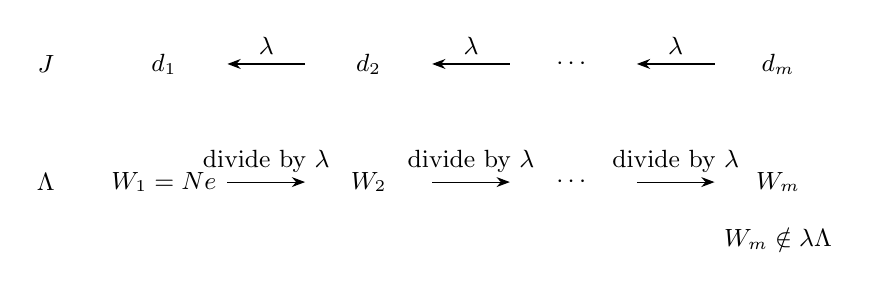
\begin{tikzpicture}[>=Stealth, every node/.style={font=\small},
                    point/.style={minimum width=1.6cm,minimum height=0.7cm}]
 \node at (-1.5,0) {$J$};
 \node at (-1.5,-1.5) {$\Lambda$};
 \node[point] (d1) at (0,0) {$d_1$};
 \node[point] (d2) at (2.6,0) {$d_2$};
 \node[point] (dd) at (5.2,0) {$\cdots$};
 \node[point] (dm) at (7.8,0) {$d_m$};
 \draw[->] (d2) -- node[above] {$\lambda$} (d1);
 \draw[->] (dd) -- node[above] {$\lambda$} (d2);
 \draw[->] (dm) -- node[above] {$\lambda$} (dd);
 \node[point] (w1) at (0,-1.5) {$W_1=Ne$};
 \node[point] (w2) at (2.6,-1.5) {$W_2$};
 \node[point] (ww) at (5.2,-1.5) {$\cdots$};
 \node[point] (wm) at (7.8,-1.5) {$W_m$};
 \draw[->] (w1) -- node[above] {divide by $\lambda$} (w2);
 \draw[->] (w2) -- node[above] {divide by $\lambda$} (ww);
 \draw[->] (ww) -- node[above] {divide by $\lambda$} (wm);
 \node[below=1mm of wm] {$W_m\notin\lambda\Lambda$};
\end{tikzpicture}
\caption{The two chains in Proposition~\ref{geom:separation}.
Tests run from left to right.  Reaching test $t$ requires
$\lambda d_t=[W_t]$; equal labels at $t<m$ give
$d_t=[W_{t+1}]$ and allow the next test.  Equal labels at the final test
would require the forbidden additional division of $W_m$ in $\Lambda$.
No equality between the rows is assumed before its test is reached.}
\label{geom:ladder}
\end{figure}

The geometric mechanism is now complete: Corollary~\ref{geom:lifts}
supplies the class $d_m$, and Proposition~\ref{geom:separation} forces
distinct labels using that class.  The next sections implement divisor
arithmetic, class division, and evaluation without recovering the roots
of $F$ or factoring the finite supports of divisors.

\section{Divisor arithmetic without factoring supports}
\label{sec:divisors}

The lifting argument uses rational divisors, although the finite points in
their supports are not given individually.  We now give a representation in
which addition, reduction, and evaluation require only polynomial arithmetic
and linear algebra.  Two further operations will be needed: summing divisors
computed simultaneously at the unknown roots of $F$, and evaluating a
principal function whose divisor has very large coefficients at infinity.
Linear-algebra algorithms for Riemann--Roch spaces and divisor arithmetic
are established tools; see Hess~\cite{Hess02} and
Khuri-Makdisi~\cite{KhuriMakdisi04}.  We give the representation and size
bounds explicitly because both the genus and the degree of the cover vary
in this application.

Throughout this section, $k$ is a finite field, $q$ is an odd prime different
from its characteristic, $k$ contains a specified primitive $q$th root
$\zeta$, and $F\in k[X]$ is monic and square-free of degree $N\geq q$, with
$q\mid N$.  We use the curve, automorphism, and rational points at infinity
introduced above.  Thus
\[
 C:\ Y^q=F(X),\qquad
 \mathcal L=k(C),\qquad
 O=k[X,Y]/(Y^q-F(X)),\qquad
 g=\frac{(q-1)(N-2)}2.
\]
The automorphism $\sigma$ sends points by $Y\mapsto\zeta Y$ and acts on
functions by $Y\mapsto\zeta^{-1}Y$.  All divisors in the computation are
$k$-rational divisors, written as sums of closed points.  For a divisor $D$,
write
\[
 \|D\|=\sum_P |v_P(D)|[k(P):k]
\]
for its absolute degree.  Bounds polynomial in $\|D\|$ do not mean bounds
polynomial in the bit length of arbitrary divisor coefficients.  Large
coefficients supported at infinity are treated separately at the end of
this section.

\begin{proposition}[Effective divisor arithmetic]\label{div:arithmetic}
On the curve $C$ above, the following operations are deterministic and use
a number of field operations polynomial in $q,N$, the degrees occurring in
the input representation, the absolute degrees of the divisors
materialized during the operation, and the parameter $\ell$ in the third
operation:
\begin{enumerate}
 \item divisor addition, negation, coefficientwise minimum and maximum,
 and the action of $\sigma$;
 \item construction of the divisor of an explicitly represented nonzero
 function, and evaluation of its valuation and leading coefficient at a
 specified ramification point or point at infinity;
 \item computation of the Riemann--Roch space
 $L(D+\ell\infty_0)$ for $\ell\geq 0$;
 \item replacement of a degree-zero divisor $D$ by a linearly equivalent
 divisor $D'$ satisfying $\|D'\|\leq 2g$, with a function $a$ such that
 $D'=D+\operatorname{div}(a)$.
\end{enumerate}
These algorithms do not require factorization of the polynomials defining
the finite supports.  Their decisions use only field zero tests, so they
admit simultaneous execution as in Lemma~\ref{ff:simultaneous}.
\end{proposition}

We prove the proposition by constructing the algorithms.  The final two
subsections extend them to simultaneous sums and to binary infinity
coefficients.

\subsection{Fractional ideals and finite linear algebra}

Smoothness of the affine curve implies that $O$ is a Dedekind domain.  It is
a free $k[X]$-module with basis $1,Y,\ldots,Y^{q-1}$.  The finite part of a
divisor $D$ is represented by the fractional ideal
\begin{equation}\label{div:ideal}
 I(D)=\{a\in\mathcal L:v_P(a)\geq v_P(D)
                 \text{ at every finite point }P\}.
\end{equation}
The zero function is included in this definition.  The rest of the
representation is the integer vector
$(v_{\infty_0}(D),\ldots,v_{\infty_{q-1}}(D))$.

To store a fractional ideal $I$, choose a monic polynomial $H\in k[X]$
such that
\begin{equation}\label{div:bound}
 HO\subseteq I\subseteq H^{-1}O.
\end{equation}
Store the image of $I$ as a $k$-subspace of $H^{-1}O/HO$.  Multiplication
by $H$ identifies this quotient with $O/H^2O$, of dimension $2q\deg H$.
Thus a subspace basis consists of polynomial vectors modulo $H^2$ in the
standard $Y$-basis.  Lifting this basis and adjoining $H$ gives a finite
list of $O$-generators of $I$.  Conversely, from such generators and a
bound~\eqref{div:bound}, take their images and repeatedly enlarge their
$k$-span under multiplication by $X$ and $Y$.  The process stabilizes in
at most $2q\deg H$ strict enlargements and gives the required ideal image.
The convention $H=1$ represents $I=O$ with a zero-dimensional quotient.

The identities
\begin{align*}
 I(D+E)&=I(D)I(E),& I(-D)&=I(D)^{-1},\\
 I(\min(D,E))&=I(D)+I(E),&
 I(\max(D,E))&=I(D)\cap I(E)
\end{align*}
reduce the first group of operations to finite linear algebra.  For a
product, take pairwise products of generators and use the bound $H_DH_E$.
For a sum or intersection, embed both subspaces using that same common
bound, and take their sum or intersection.  For inversion, retain the
bound $H$: an element $a\in H^{-1}O$ belongs to $I^{-1}$ precisely when
$au\in O$ for every generator $u$ of $I$.  These are linear conditions
on $H^{-1}O/HO$.  They are independent of the chosen representative of $a$,
since $HI\subseteq O$.  The action of $\sigma$ is substitution of
$\zeta^{-1}Y$ for $Y$ in the generators.  The corresponding operations on
the infinity vectors are immediate.

A known ramification point $P=(x,0)$ has ideal $(X-x,Y)$, with bound
$H=X-x$.  For a nonzero function $a$, arithmetic in $\mathcal L$ uses
rational coefficients in $k(X)$ in the standard $Y$-basis.  Inversion is
linear algebra over $k(X)$.  Clearing denominators in both $a$ and $a^{-1}$
gives a polynomial $H$ for which $aO$ satisfies~\eqref{div:bound}; hence
the finite part of $\operatorname{div}(a)$ is computable without finding
any of its points.

Intermediate bound polynomials need not be minimal.  The following
compression both controls their degrees and supplies the norm data used
in class division.

\begin{lemma}[Compression and pushforward]\label{div:compression}
From the representation of $I=I(D)$ one can compute monic polynomials
$h^+,h^-\in k[X]$ satisfying
\[
 \deg h^+=\sum_{P\text{ finite}}\max(v_P(D),0)[k(P):k],\qquad
 \deg h^-=\sum_{P\text{ finite}}\max(-v_P(D),0)[k(P):k].
\]
The polynomial $H=h^+h^-$ satisfies~\eqref{div:bound}.  If $\deg D=0$ and
$j=h^+/h^-$, then
\begin{equation}\label{div:orbitnorm}
 \operatorname{div}_C(j)=\sum_{a=0}^{q-1}\sigma^aD.
\end{equation}
\end{lemma}

\begin{proof}
Form the integral ideals
$I^+=I\cap O$ and $I^-=I^{-1}\cap O$.  Let $h^+$ and $h^-$ be the
characteristic polynomials of multiplication by $X$ on $O/I^+$ and
$O/I^-$, respectively.  These quotients are computed from the stored
subspaces; the original bound $H_0$ has $H_0O\subseteq I^+,I^-$, so it
suffices to work in $O/H_0O$.  A quotient at a closed point $P$ of
multiplicity $d$ has a filtration with $d$ successive residue fields
$k(P)$.  Its $k$-dimension is therefore $d[k(P):k]$, proving the degree
formulas.

Cayley--Hamilton gives $h^+O\subseteq I^+\subseteq I$ and
$h^-O\subseteq I^-\subseteq I^{-1}$.  The second inclusion implies
$I\subseteq(h^-)^{-1}O$.  Both sides of~\eqref{div:bound} now follow
for $H=h^+h^-$.  Recompute the ideal subspace with this bound after each
operation.  In particular, its dimension is at most twice $q$ times the
absolute degree of the finite divisor.

For the last assertion, let $Q=X(P)$ be a finite point downstairs and
$f_Q$ its monic defining polynomial.  On $k(P)$, multiplication by $X$
has characteristic polynomial $f_Q^{[k(P):k(Q)]}$.  Applying this fact to
the preceding filtrations shows that the finite divisor of $j$ on
$\mathbb P^1$ is $X_*D$ at the finite points.  Since $\deg D=0$, the
infinity coefficient agrees as well.  Finally, for this cyclic cover,
$X^*X_*D=\sum_{a=0}^{q-1}\sigma^aD$, including the ramified points and
points with nontrivial residue extension.  This proves
\eqref{div:orbitnorm}.
\end{proof}

\subsection{Local expansions and Riemann--Roch reduction}

The ideal representation controls all finite points collectively.  At the
few specified points where a value or inequality is required, local
expansions give the additional information.

At infinity use $z=X^{-1}$ and $U=Yz^{N/q}$.  The equation
\[
 U^q=z^NF(z^{-1}),\qquad U(0)=\zeta^j
\]
determines the expansion at $\infty_j$ by simple-root Hensel lifting.
At $P=(x,0)$ use $Y$ as uniformizer and solve $F(X)=Y^q$ with $X(0)=x$;
the derivative $F'(x)\ne0$ again permits coefficient-by-coefficient
lifting.  The valuation and leading coefficient of a nonzero function
are then found by substitution and division of the leading terms.

Here is an explicit precision bound.  Write a function as
$A(X,Y)/B(X)$, where $\deg_Y A<q$ and every coefficient in $X$, as well
as $B$, has degree at most $E$.  The polynomial $A$ has poles only at
infinity, with total pole degree at most $q(E+N)$; the same bound holds
for $B$.  The degree of its zero divisor equals its pole degree, so no
nonzero numerator or denominator can have an order of vanishing greater
than this bound at a rational point.  Consequently local substitutions
through precision
\begin{equation}\label{div:precision}
 8q(E+N+1)
\end{equation}
suffice to identify their first nonzero Laurent coefficients, even after
the possible pole at infinity has been removed.  For a represented
divisor, its coefficient at a specified finite point is the minimum of
the valuations of a list of ideal generators; zero generators may be
discarded.

We next turn Riemann--Roch existence into a linear computation.  Recall
that
\[
 L(V)=\{a\in\mathcal L:\operatorname{div}(a)+V\geq0\}\cup\{0\}
\]
is a finite-dimensional $k$-vector space.  Given $D$ and $\ell\geq0$,
choose a bound $H$ for $I(-D)$.  Every function in $L(D+\ell\infty_0)$
has the form
\begin{equation}\label{div:rransatz}
 a=H^{-1}\sum_{j=0}^{q-1}a_j(X)Y^j,
 \qquad \deg a_j\leq \deg H+\|D\|+\ell.
\end{equation}
To justify the degree bound, put
\[
 M=\max_{a_j\ne0}\bigl(\deg a_j+jN/q-\deg H\bigr).
\]
The coefficient of $z^{-M}$ in the expansions at infinity is a nonzero
polynomial of degree less than $q$ evaluated at the $q$ distinct values
$1,\zeta,\ldots,\zeta^{q-1}$.  It cannot vanish at all of them.  Thus
at one infinity point the pole order, interpreted as $-v_{\infty_j}(a)$,
is exactly $M$.  The defining inequalities for $L(D+\ell\infty_0)$ give
$M\leq\|D\|+\ell$, which implies~\eqref{div:rransatz}.

In this finite ansatz, membership in $I(-D)$ is a subspace condition, and
\[
 v_{\infty_j}(a)\geq-v_{\infty_j}(D)-\ell\,\mathbf1_{j=0}
 \qquad(0\leq j<q)
\]
is a list of linear conditions on Laurent coefficients.  Expansions to
the bound~\eqref{div:precision}, increased by
$8q(\|D\|+\ell+1)$, suffice.  Solving the resulting linear system
therefore computes the whole space $L(D+\ell\infty_0)$.

For degree-zero $D$, the Riemann--Roch inequality
\cite[Tag~0BS6]{StacksProject} gives
$\dim_kL(D+g\infty_0)\geq1$.  Choose a nonzero solution $a$ by a fixed
pivot convention and define
\begin{equation}\label{div:reduce}
 \operatorname{ReduceDivisor}(D)=D'=D+\operatorname{div}(a).
\end{equation}
Since $D'+g\infty_0$ is effective of degree $g$, we have
$\|D'\|\leq2g$.  Retain $a$ whenever a later computation needs the
linear equivalence.  If a degree-zero divisor $D$ is known to be
principal, taking $\ell=0$ instead produces a nonzero $a$ with
$D+\operatorname{div}(a)=0$: the effective divisor on the left has degree
zero.

All vector spaces and polynomial degrees in these constructions are
polynomial in the parameters in Proposition~\ref{div:arithmetic}.
Dense polynomial operations, fraction reduction over $k(X)$, and linear
algebra therefore prove its complexity assertion.  For example, the
ideal quotient has dimension $2q\deg H$, and the ansatz
\eqref{div:rransatz} has at most
$q(\deg H+\|D\|+\ell+1)$ unknowns.  Rational linear algebra does not
cause uncontrolled degree growth: after common denominators are cleared,
minors of an $s\times s$ matrix with polynomial entries of degree at
most $d$ have degree at most $sd$.  Reduced elimination entries and
solutions are ratios of such minors.  This completes the proof of
Proposition~\ref{div:arithmetic}.

\subsection{Summing divisors given over a product algebra}

The odd-degree splitter first produces one divisor for each root of $F$,
through a computation over $A=k[T]/F(T)$.  The next lemma computes their
sum over $k$, while the roots remain unknown.  A norm from the finite
algebra $A$ will replace the unavailable product over its components.

\begin{lemma}[Simultaneous divisor sum]\label{div:trace}
Suppose $A\simeq k^s$ is an explicitly represented split algebra.  Let
$I_1,\ldots,I_s$ be fractional ideals of $O$ supplied together over $A$,
with monic bounds $H_i$ and a common number $b$ of generators
$u_{i0},\ldots,u_{i,b-1}$, including $H_i$.  If the prime subfield
contains more than $s(b-1)$ elements, their product can be computed by
polynomial arithmetic, determinants, and ideal closure, without a
decomposition of $A$.  Together with addition of the infinity vectors,
this computes the sum of the corresponding divisors.
\end{lemma}

\begin{proof}
Let $H\in A[X]$ denote the tuple of bounds and let $u_j$ denote the tuple
of $j$th generators.  Form
\[
 H_* =\operatorname{Norm}_{A/k}(H)=\prod_{i=1}^s H_i,
 \qquad
 w_a=\operatorname{Norm}_{A/k}\left(\sum_{j=0}^{b-1}a^ju_j\right)
     =\prod_{i=1}^s\left(\sum_{j=0}^{b-1}a^ju_{ij}\right).
\]
The norm is the determinant of multiplication after extending scalars
to the relevant polynomial or function ring.  The displayed products
are identities proving correctness, not instructions to recover the
components.  Denominators are cleared by multiplying the $i$th component
by $H_i$; the resulting determinant lies in $O$, and division by $H_*$
recovers $w_a$.  Polynomial determinants can be computed before reducing
by $Y^q-F(X)$.  Use $s(b-1)+1$ distinct values of $a$ from the prime
subfield.

Each $w_a$ belongs to $\prod_i I_i$.  Fix a finite closed point $P$ and
write $d_i=\min_jv_P(u_{ij})$.  After dividing the $i$th combination by
a local uniformizer to power $d_i$, its residue is a nonzero polynomial
in $a$, over $k(P)$, of degree at most $b-1$.  At most $b-1$ of our
values fail to attain valuation $d_i$.  Thus some chosen $a$ attains all
$d_i$ simultaneously, and $v_P(w_a)=\sum_i d_i$.  Fractional ideals in
a Dedekind domain are determined by these minimum valuations.  The
$w_a$ therefore generate exactly $\prod_i I_i$.  The polynomial $H_*$
is a valid bound, so finite ideal closure computes its stored
representation.

Infinity coefficients are integers.  In a simultaneous field execution
they are the same in every surviving component: any different outcome
of a scalar zero test would already have supplied a factor.  Their sum
is therefore obtained by multiplying the common vector by $s$.  More
generally, if the computation has retained separate pieces, sum their
vectors with the corresponding dimensions.
\end{proof}

For the application $s=N$.  The number $b$ can be bounded by
$2q\deg H_i+1$ in the compressed representation, and the characteristic
cutoff in Section~\ref{sec:complexity} guarantees the required distinct
scalars.  Matrix determinants and ideal closure have sizes polynomial
in these parameters.

\subsection{Binary coefficients at infinity and function circuits}

Riemann--Roch reduction has cost polynomial in absolute degree.  It must
not be applied directly to an infinity divisor whose coefficients are
exponentially large integers.  We instead perform the class arithmetic
by binary additions and retain the accompanying rational function as a
circuit.

\begin{lemma}[Principal functions with large infinity coefficients]
\label{div:circuits}
Let $D$ be a represented degree-zero divisor of bounded absolute degree,
and let $W=\sum_jw_j\infty_j$ have degree zero, with integer coefficients
given in binary.  If
$Z=(1-\sigma)D-W$ is principal, a circuit for a function $h$ satisfying
$\operatorname{div}(h)=Z$ can be computed using a number of operations
polynomial in $q,N,\|D\|$, the representation size, and
$\max_j\log(2+|w_j|)$.  The circuit uses multiplication and inversion
of explicitly represented small functions.  At each known ramification
point $P$, it computes the nonzero value $h(P)$ within the same type of
bound, without expanding $h$.
\end{lemma}

\begin{proof}
Write $W=\sum_{j=1}^{q-1}w_j(\infty_j-\infty_0)$.  Build the divisor
$Z$ from $(1-\sigma)D$ and these signed multiples by binary doubling
and addition.  At every stage retain a reduced divisor $D_0$ and a
function circuit $w$ with the invariant
\begin{equation}\label{div:circuitinvariant}
 D_0=D_{\mathrm{target}}+\operatorname{div}(w).
\end{equation}
On adding two stages, reduce $D_1+D_2$ with reducing function $u$ and
replace the function circuit by $w_1w_2u$.  For doubling it becomes
$w_1^2u$; negation uses inversion followed, if needed, by reduction.
After the initial reduction, each materialized sum has absolute degree
at most $4g$, and the number of reductions is
$O(q\max_j\log(2+|w_j|))$, in addition to the initial operations on $D$.

At the end obtain a small divisor $\widetilde Z=Z+\operatorname{div}(w)$.
It is principal, so the $\ell=0$ Riemann--Roch computation gives $a$ with
$\widetilde Z+\operatorname{div}(a)=0$.  Consequently
\[
 h=(aw)^{-1}
\]
has divisor $Z$.  All leaves of this circuit are functions produced by
reductions on small divisors and hence have polynomial representation
size.

At $P$, expand each leaf and store its integer valuation and its nonzero
leading coefficient.  Multiplication adds valuations and multiplies
leading coefficients; inversion negates valuations and inverts leading
coefficients.  The resulting integers have bit length polynomial in the
circuit length and leaf bounds.  Because $P$ is fixed by $\sigma$ and
$W$ is supported at infinity, $v_P(Z)=0$.  The final valuation is
therefore zero, and the final leading coefficient is exactly $h(P)$.
This also explains why the intermediate objects are leading coefficients
of Laurent series, rather than values of functions that may have poles.
\end{proof}

\section{Solving the promised norm equations}
\label{sec:norms}

Division of divisor classes will require a function with a prescribed
norm.  This section constructs such a function when its existence is
known.  The construction uses linear algebra and extraction of roots in
finite reduced algebras, and its complexity is polynomial in the degree
of the cover.  In particular, the cover degree is not treated as a
constant.

\begin{theorem}[Promised norm solver]\label{norm:solve}
Let $k$ be an explicitly represented finite field of characteristic $p$,
let $q$ be an odd prime, and suppose that a primitive $q$th root of unity
$\zeta\in k$ and a generator of the full $q$-primary subgroup of $k^*$
are given.  Let $F\in k[X]$ be monic and square-free, of positive degree
$N$ divisible by $q$.  Put
\[
 K_0=k(X),\qquad
 \mathcal L=K_0[Y]/(Y^q-F),\qquad \rho(Y)=\zeta Y.
\]
Let $G\in K_0^*$, write $D$ for the maximum of its reduced numerator
and denominator degrees, and assume
\begin{equation}\label{norm:characteristic}
 p>(N+2D+1)^2.
\end{equation}
If $G$ belongs to $\operatorname{Norm}_{\mathcal L/K_0}(\mathcal L^*)$, a deterministic
algorithm constructs $h\in \mathcal L^*$ with
\[
 \prod_{j=0}^{q-1}\rho^j(h)=G.
\]
Its bit complexity, and the degrees of the rational coefficients of
$h$ in the basis $1,Y,\ldots,Y^{q-1}$, are bounded by fixed polynomials
in $q,N,D$, and $\log|k|$.  It uses no polynomial factorization oracle.
Its field-dependent branches use only zero tests, so the algorithm
admits the simultaneous execution of Lemma~\ref{ff:simultaneous}.
\end{theorem}

The characteristic bound is a convenient sufficient condition for the
scalar searches in Lemma~\ref{ff:unitroot}; the main algorithm satisfies
it with considerable room.  The roots of $F$ need not be supplied, and
the norm solver does not require $F$ to split over $k$.
The function automorphism $\rho$ is the inverse of the action $\sigma$
used in the divisor sections. Their powers run over the same cyclic
group, so they define the same norm.

We first turn the norm equation into the problem of constructing a
rank-one idempotent in an algebra.  We then obtain that idempotent from
spaces of matrices regular at the places of the rational function
field.  This use of intersections of maximal orders is closely related
to the explicit matrix-algebra algorithms of
Ivanyos--Kutas--R\'onyai~\cite{IKR18}.  Their general algorithm permits a
finite-field factorization oracle.  Here the cyclic presentation
allows the local orders to be written explicitly, and a fiber
calculation supplies the idempotent by linear algebra.  We give the
construction and its bounds in full.

\subsection{The cyclic algebra and its local matrix models}

The polynomial $Y^q-F$ is irreducible over $K_0$: a place at which $F$
has valuation one is Eisenstein for it.  Thus $\mathcal L$ is a field, cyclic of
degree $q$ over $K_0$.  Form the $K_0$-algebra
\begin{equation}\label{norm:cyclic-algebra}
 \mathcal E=\bigoplus_{b=0}^{q-1} \mathcal L V^b,
 \qquad V a=\rho(a)V\ (a\in \mathcal L),\qquad V^q=G.
\end{equation}
Its multiplication table in the basis
\[
 W_{ab}=Y^aV^b,\qquad 0\le a,b<q,
\]
is explicit.  The norm promise implies that $\mathcal E$ is a full
matrix algebra over $K_0$, but does not initially give us an
isomorphism.  Indeed, if $h_0$ is any norm solution, let $\mathcal L$ act on
itself by multiplication and let $V$ act by $h_0\rho$.  These operators
satisfy \eqref{norm:cyclic-algebra}.  Their linear independence follows
by applying a putative relation between the operators $\rho^b$ to
$1,Y,\ldots,Y^{q-1}$ and using the invertible matrix
$(\zeta^{bj})_{b,j}$.  Dimension then gives an isomorphism
\begin{equation}\label{norm:abstract-splitting}
 \mathcal E\simeq M_q(K_0).
\end{equation}
This argument establishes existence only; the algorithm never uses
$h_0$ or this unspecified isomorphism.

A \emph{rank-one idempotent} in $\mathcal E$ is an element $e$ with
$e^2=e$ whose image under \eqref{norm:abstract-splitting} has rank one.
The following observation explains why constructing such an element
solves the original norm equation.

\begin{lemma}\label{norm:idempotent-to-norm}
Given a rank-one idempotent $e\in\mathcal E$, linear algebra over
$K_0$ constructs a norm solution $h\in \mathcal L$.
\end{lemma}

\begin{proof}
The left ideal $\mathcal E e$ has dimension $q$ over $K_0$.  The map
$\mathcal L\to\mathcal E e$, $a\mapsto ae$, is injective, since any nonzero
$a\in \mathcal L$ is invertible.  Both sides have dimension $q$, so it is an
isomorphism.  In particular, there is a unique $h\in \mathcal L$ satisfying
\begin{equation}\label{norm:extract-h}
 Ve=he.
\end{equation}
Solve this equation for the $q$ coefficients of $h$ in the basis
$1,Y,\ldots,Y^{q-1}$, using the explicit $q^2$-element basis of
$\mathcal E$ to express both sides.  Repeatedly multiply the equation
on the left by $V$, using $Va=\rho(a)V$.  After $q$ steps this gives
\[
 G e=V^q e=\left(\prod_{j=0}^{q-1}\rho^j(h)\right)e.
\]
Since $e\ne0$ and the two coefficients are scalars in $K_0$, their
equality proves the norm equation.  In particular $h\ne0$.
\end{proof}

Our remaining task is to construct $e$.  We will impose local
integrality conditions on elements of $\mathcal E$, then find a
rank-one matrix in their values at infinity.

Let $v$ be a closed point of $\mathbb P^1_k$.  Write $K_v$ for the
completed rational function field, $R_v$ for its valuation ring,
$\kappa_v$ for its residue field, and $T$ for a uniformizer.  A
\emph{lattice} in a finite-dimensional $K_v$-space is a free $R_v$-module
of full rank.  An \emph{order} in $\mathcal E\otimes K_v$ is a lattice
that contains $1$ and is closed under multiplication; it is
\emph{maximal} if no strictly larger order contains it.  We construct
one maximal order $\mathcal A_v$ at every $v$.  Only the points dividing
$F$, the numerator or denominator of $G$, and the point at infinity
require nontrivial conditions.

We will repeatedly use the matrix trace $\operatorname{tr}$ on the
split algebra.  It does not depend on the choice of isomorphism in
\eqref{norm:abstract-splitting}.  Conjugation by $Y$ and $V$ shows that
every nonidentity basis monomial has trace zero, while
$\operatorname{tr}(1)=q$.  Consequently
\begin{equation}\label{norm:trace-coordinates}
 a=\sum_{a',b'} c_{a'b'}W_{a'b'}
 \quad\Longrightarrow\quad
 c_{ab}=q^{-1}\operatorname{tr}(aW_{ab}^{-1}).
\end{equation}
Here $q$ is invertible by \eqref{norm:characteristic}.

\paragraph{Unramified places with $q\mid v(G)$.}
Suppose $v$ is finite, $v(F)=0$, and $w=v(G)$ is divisible by $q$.
Set $\widetilde V=T^{-w/q}V$, and take the $R_v$-span of
$Y^a\widetilde V^b$.  Both $Y$ and $\widetilde V$ have unit $q$th
powers, so this span is an order and contains the inverses of all its
basis monomials.  It is maximal.  To see this, any larger order has
integral matrix traces: its regular left-action trace is integral and
equals $q$ times matrix trace.  Pairing an element of the larger order
with the inverse basis monomials in
\eqref{norm:trace-coordinates} therefore makes all its coordinates
integral.  It already belongs to the displayed span.  This description
applies at all finite places outside the indicated finite set, with
$w=0$.

\paragraph{Places ramified in $\mathcal L$.}
Suppose $v(F)=1$, and again put $w=v(G)$.  Since $q$ is odd,
\begin{equation}\label{norm:ramified-unit}
 V'=Y^{-w}V,\qquad (V')^q=u:=G/F^w\in R_v^*.
\end{equation}
The commutation factor in taking the $q$th power is a power of
$\zeta^{q(q-1)/2}=1$.  The residue of $u$ is a $q$th power in
$\kappa_v^*$.  Indeed the extension at $v$ is totally ramified of
degree $q$.  For any promised solution $h_0$ one has
$v_{\mathcal L}(h_0)=v(G)=w$, with $v_{\mathcal L}(Y)=1$.  Hence $h_0/Y^w$ is a unit, its
norm is $u$, and the residue of that norm is the $q$th power of its
residue.

Take a residue root and lift it by Hensel's method to $R\in R_v^*$
with $R^q=u$.  On column vectors $e_0,\ldots,e_{q-1}$ define
\begin{equation}\label{norm:ramified-matrices}
 V'e_j=\zeta^jR e_j,\qquad
 Ye_j=\begin{cases}e_{j+1},&j<q-1,\\F e_0,&j=q-1.\end{cases}
\end{equation}
These matrices satisfy $V'Y=\zeta YV'$, $Y^q=F$, and $(V')^q=u$.
The distinct diagonal entries of $V'$ give all diagonal matrix units
by interpolation, and the invertible shift $Y$ gives the remaining
matrix units over $K_v$.  Thus the model is an isomorphism to
$M_q(K_v)$.  Let $\mathcal A_v$ be the inverse image of $M_q(R_v)$.

\paragraph{Unramified places with $q\nmid v(G)$.}
Suppose $v(F)=0$ and $q\nmid w=v(G)$.  The residue of $F$ must be a
$q$th power.  Otherwise, since $\kappa_v$ contains $\mu_q$ and $q$ is
prime, $Y^q-\overline F$ is irreducible and defines an unramified
extension of degree $q$.  All its norm valuations are then divisible
by $q$, contradicting the promise on $G$.  Lift a residue root to
$S\in R_v^*$ with $S^q=F$.  Use the matrices
\begin{equation}\label{norm:unramified-matrices}
 Ye_j=\zeta^{-j}S e_j,\qquad
 Ve_j=\begin{cases}e_{j+1},&j<q-1,\\G e_0,&j=q-1.\end{cases}
\end{equation}
Now $VY=\zeta YV$, including at the wrap from $e_{q-1}$ to $e_0$.
The same matrix-unit argument gives an isomorphism to $M_q(K_v)$;
again take the inverse image of $M_q(R_v)$.

\paragraph{Infinity.}
Put $z=X^{-1}$ and $\widetilde Y=z^{N/q}Y$.  Then
\[
 \widetilde Y^q=z^NF(z^{-1})=:F_\infty(z),\qquad F_\infty(0)=1.
\]
There is a unique root $S\in k[[z]]$ of $S^q=F_\infty$ with $S(0)=1$.
Use \eqref{norm:unramified-matrices} with $\widetilde Y$ in place of
$Y$, and with the same weighted shift for $V$, whatever the valuation
of $G$ may be.  The inverse image of $M_q(k[[z]])$ is $\mathcal A_\infty$.
This model also specifies reduction to $M_q(k)$ at infinity.

The matrix orders just used are maximal.  For example, pairing with
matrix units shows that any element in a larger order has integral
matrix entries, using the integrality of matrix trace exactly as
above.  We have therefore specified maximal orders at every place,
using only residue roots whose existence follows from the norm
promise.

\subsection{Why one fiber contains a rank-one matrix}

Define the finite-dimensional $k$-algebra of global sections and its
evaluation image by
\begin{equation}\label{norm:sections-fiber}
 \mathcal S=\{a\in\mathcal E:a\in\mathcal A_v\text{ for every }v\},
 \qquad
 \mathcal B=\operatorname{ev}_\infty(\mathcal S)\subseteq M_q(k).
\end{equation}
We will compute both spaces by linear equations.  First we establish
the feature of $\mathcal B$ that will make this useful: up to change of
basis it is the algebra of all block upper triangular matrices.  Its
first block therefore contains the image of a rank-one idempotent.

Here is the geometric explanation, including the descent from
completed local orders.  Intersect $\mathcal A_v$ with the rational
algebra $\mathcal E$.  This is a full lattice over the ordinary local
discrete valuation ring at $v$, and its completion is
$\mathcal A_v$.  Indeed the completed lattice lies between two powers
of a rational uniformizer times a fixed rational lattice.  Rational
approximation to a basis, to sufficiently high precision, produces a
basis of the same completed lattice.  Equivalently, the finitely many
congruences between these two bounds descend to the ordinary local
ring.  Maximality descends as well, since a larger ordinary order
would yield a larger completed order.

For the following existence argument only, fix an isomorphism
\eqref{norm:abstract-splitting}.  An ordinary local maximal order in
$M_q(K_0)$ is the endomorphism ring of a lattice.  In fact, apply the
order to the standard local lattice $R^q$ and take its span $M$.
The order is a finite module and contains the identity, so $M$ is a
full lattice stable under it.  The containing order
$\operatorname{End}_R(M)$ must equal it by maximality.  At all but
finitely many places the standard rational basis matrices and their
inverse change of coordinates are integral; there we may use $M=R^q$.
The resulting lattices glue to a vector bundle $\mathcal V$ of rank
$q$ on $\mathbb P^1_k$.  Concretely, its local sections are rational
column vectors satisfying the specified lattice conditions.  A basis
of one local lattice gives a trivialization on a neighborhood after
excluding the finitely many poles and other exceptional points.
We have proved
\begin{equation}\label{norm:endomorphism-bundle}
 \mathcal S=H^0(\mathbb P^1_k,\operatorname{End}\mathcal V).
\end{equation}
The chosen matrix model at infinity identifies the endomorphism
fiber with $M_q(k)$.  Any two such identifications differ by
conjugation: an automorphism of a full matrix algebra sends matrix
units to matrix units, from which a change of column basis is
obtained.  Thus its particular choice will not affect the asserted
shape of $\mathcal B$.

The following form of the projective-line splitting theorem holds
over the original field, rather than only after extending its
constants; see Hazewinkel--Martin~\cite{HazewinkelMartin82}.

\begin{lemma}[Splitting on the projective line]\label{norm:bundle-split}
Every vector bundle on $\mathbb P^1_k$ is a direct sum of line bundles
$\mathcal O(d)$, with integer degrees $d$.
\end{lemma}

\begin{proof}
We recall a proof over the given field $k$.  Line bundles on
$\mathbb P^1_k$ are classified by their degree.  On the two standard
affine charts, the Laurent-polynomial computation of their
cohomology gives
\[
 H^0(\mathcal O(t))=0\ (t<0),\qquad
 H^1(\mathcal O(t))=0\ (t\ge-1).
\]
The first assertion is immediate from polynomial degrees; for the
second, the \v Cech quotient is spanned by the Laurent monomials
between the two chart ranges, and that range is empty for $t\ge-1$.

Choose the largest integer $d$ for which there is a nonzero map
$\mathcal O(d)\to\mathcal V$.  Such integers exist and are bounded
above: enclosing the finitely many defining lattices of $\mathcal V$
between twists of a fixed trivial bundle proves both claims.  A
nonzero map is generically injective.  Saturating its image would
increase its degree by the effective divisor of its zeros, so
maximality of $d$ implies that it is a line subbundle.  The quotient
$\mathcal Q$ is a vector bundle, and induction on rank writes it as
$\bigoplus_i\mathcal O(t_i)$.  Twist
\[
 0\longrightarrow\mathcal O(d)\longrightarrow\mathcal V
   \longrightarrow\mathcal Q\longrightarrow0
\]
by $-d-1$.  Maximality of $d$ gives
$H^0(\mathcal V(-d-1))=0$, and $H^1(\mathcal O(-1))=0$.
The cohomology sequence therefore gives
$H^0(\mathcal Q(-d-1))=0$, whence $t_i\le d$ for every $i$.
Finally, each extension group
\[
 \operatorname{Ext}^1(\mathcal O(t_i),\mathcal O(d))
   =H^1(\mathcal O(d-t_i))
\]
vanishes.  The sequence splits, completing the induction.
\end{proof}

Apply the lemma and order the summands by decreasing degree:
$\mathcal V=\bigoplus_{i=1}^q\mathcal O(d_i)$ with
$d_1\ge\cdots\ge d_q$.  The $(i,j)$ entry of a global endomorphism
is a section of $\mathcal O(d_i-d_j)$.  If $d_i<d_j$ it is zero;
otherwise its value at infinity is arbitrary, because a line bundle
of nonnegative degree has a section with any prescribed value at that
point.  Grouping the equal degrees proves the promised block upper
triangular description of $\mathcal B$.  This is an existence proof of
the shape, not an algorithm for computing the splitting of
$\mathcal V$.

\begin{lemma}[Extracting a rank-one fiber idempotent]
\label{norm:fiber-idempotent}
Given a basis of a subalgebra $\mathcal B\subseteq M_q(k)$ that is
conjugate to a full block upper triangular algebra, linear algebra
over $k$ constructs a rank-one idempotent in $\mathcal B$.
\end{lemma}

\begin{proof}
Compute the kernel $\mathcal N$ of the bilinear form
\[
 (a,b)\longmapsto\operatorname{tr}(ab),\qquad a,b\in\mathcal B.
\]
In block upper triangular coordinates, a product has diagonal blocks
equal to the products of the corresponding diagonal blocks.  The
ordinary trace pairing on a full matrix algebra is nondegenerate in
every characteristic, as is seen by pairing its matrix units.
Hence $\mathcal N$ is exactly the strictly block upper triangular
part.  The common kernel
\[
 U=\bigcap_{n\in\mathcal N}\ker n
\]
is the column space of the first block; if there is only one block,
$\mathcal N=0$ and $U=k^q$.  Indeed every later block has arbitrary
maps to the first block, which exclude any vector with a nonzero
later component from this common kernel.

Choose $0\ne v\in U$ and a row $w$ with $wv=1$.  Then $a_0=vw$
has rank one and satisfies $a_0^2=a_0$.  In block coordinates it has
nonzero entries only in the first block row, so it belongs to
$\mathcal B$.  The computation requires only kernels and one scalar
normalization; it does not require finding the conjugating matrix.
\end{proof}

\begin{figure}[tb]
\centering
\[
 \mathcal B\sim
 \begin{pmatrix} *&*&*\\0&*&*\\0&0&*\end{pmatrix}
 \quad\xrightarrow{\ \ker\operatorname{tr}(ab)\ }\quad
 \mathcal N\sim
 \begin{pmatrix}0&*&*\\0&0&*\\0&0&0\end{pmatrix},
 \qquad
 U\sim\begin{pmatrix}k^{r_1}\\0\\0\end{pmatrix}.
\]
\caption{The fiber calculation with three distinct degree blocks.
Each star denotes an arbitrary matrix block, and the diagonal block
sizes are $r_1,r_2,r_3$.  The common kernel $U$ of the trace-pairing
kernel is the first block column space.  Every matrix $vw$ with
$v\in U$ belongs to $\mathcal B$; choosing $wv=1$ gives the rank-one
idempotent.  The calculation works in the original coordinates.}
\label{fig:norm-fiber}
\end{figure}

Figure~\ref{fig:norm-fiber} isolates the part of the vector-bundle
argument that is actually computed.  The splitting theorem guarantees
the triangular shape; the trace pairing finds enough of that shape
to construct a rank-one matrix without a factorization or a change
of basis.

\subsection{From the fiber idempotent to a norm solution}

Lift the matrix $a_0$ of Lemma~\ref{norm:fiber-idempotent} to any
$b\in\mathcal S$ with $\operatorname{ev}_\infty(b)=a_0$.  This is a
linear solve once \eqref{norm:sections-fiber} has been computed.  The
coefficients of the generic characteristic polynomial of $b$ are
regular at every point, since $b$ is a global endomorphism of
$\mathcal V$.  A rational function regular on $\mathbb P^1_k$ is
constant.  Evaluating at infinity consequently gives
\[
 \det(T-b)=T^{q-1}(T-1).
\]
The primary decomposition for the relatively prime factors
$T^{q-1}$ and $T-1$ shows that
\begin{equation}\label{norm:generic-idempotent}
 e=b^q
\end{equation}
is the projection onto the one-dimensional $1$-eigenspace: it is zero
on the nilpotent part and the identity on that eigenspace.  Thus $e$
is a rank-one idempotent in $\mathcal E$.

Lemma~\ref{norm:idempotent-to-norm} now recovers a norm solution by
solving $Ve=he$ over $K_0$.

It remains to make the spaces in \eqref{norm:sections-fiber}
computable with polynomially many coefficients.  This is where the
explicit local models, rather than an unspecified splitting of the
cyclic algebra, are essential.

\subsection{Computing all sections by finite linear systems}
\label{norm:section-computation}

Write $G=A/B$ with coprime nonzero polynomials $A,B\in k[X]$.
Square-free decomposition and gcds partition the finite places
dividing $FAB$ into pairwise coprime monic square-free polynomials
$H_i$ such that the two values
\[
 \bigl(v(F),v(G)\bigr)=(\epsilon_i,w_i)
\]
are constant over the irreducible factors of each $H_i$.
No irreducible factorization is involved: decompose the multiplicity
layers of $A$ and $B$ and refine their intersections with each other
and with $F$ by gcds.  All these polynomials have degree less than
$p$ by \eqref{norm:characteristic}, so derivative-based square-free
decomposition has no inseparable residual case.  Put
\begin{equation}\label{norm:H-M}
 H=\prod_i H_i,\qquad d_H=\deg H\le N+2D,
 \qquad M=10q^2(N+D+1).
\end{equation}

At every place in group $i$ we may use the same rational uniformizer
$T=H_i$.  Arithmetic modulo $H_i^s$ carries out, simultaneously, all
the required arithmetic modulo the $s$th power of these local
uniformizers.  The Chinese remainder theorem explains this statement
without requiring the factors of $H_i$ to be computed.  When a local
model requires a residue root, its residue is a unit modulo $H_i$
and is a $q$th power in every residue-field component by the norm
promise.  Lemma~\ref{ff:unitroot} constructs the root in $k[X]/H_i$.
The characteristic bound supplies more than $d_H^2$ distinct prime
field scalars for that lemma.  Hensel lifting then works modulo powers
of $H_i$, since the derivative $qR^{q-1}$ or $qS^{q-1}$ is a unit.

\begin{lemma}[Bounds for the local models]\label{norm:local-bounds}
At a place with one of the matrix models above, every nonzero entry
of the matrices of $W_{ab}$ and $W_{ab}^{-1}$ has valuation between
$-M$ and $M$.  At a place with the scaled-basis order, the exponents
changing between that basis and $W_{ab}$ have absolute value at most
$M$.  Consequently, the standard coefficients of every local-order
element have valuation at least $-M$ at the exceptional places and
at infinity.  At all other finite places those coefficients are
integral.
\end{lemma}

\begin{proof}
At a ramified finite place, let $D_R$ denote the unit diagonal matrix
of $V'$.  Then $V=Y^wD_R$, and commutation gives
\[
 W_{ab}=\zeta^{wb(b-1)/2}Y^{a+wb}D_R^b.
\]
For any integer $t$, the nonzero entry of $Y^t$ in column $j$ has
valuation $\lfloor(j+t)/q\rfloor$.  Since $0\le a,b<q$ and
$|w|\le D$, these valuations, and those of the inverse matrices,
have absolute value at most $D+2$.  In the unramified matrix model,
$Y$ is a unit diagonal matrix and each entry of $V^b$, for $b<q$,
has valuation either $0$ or $w$; inverse entries have the opposite
valuations.  At infinity the extra factor $z^{-aN/q}$ in $Y^a$
gives the bound $N+D$.  These bounds are smaller than $M$.
In the scaled-basis case, the change is multiplication by
$T^{\pm bw/q}$, whose exponent has absolute value at most $D$.

For an element in a matrix order, formula
\eqref{norm:trace-coordinates} and the bound on the inverse basis
matrices give the coefficient bound $-M$.  The scaled-basis assertion
gives the same conclusion in the remaining case.  At an ordinary
finite place the order is the unscaled standard span, so the
coefficients are integral there.
\end{proof}

It follows that every global section is included in the ansatz
\begin{equation}\label{norm:ansatz}
 b=\sum_{a,b'=0}^{q-1}c_{ab'}W_{ab'},\qquad
 c_{ab'}=\frac{P_{ab'}(X)}{H(X)^M},\qquad
 \deg P_{ab'}\le M(d_H+1).
\end{equation}
Indeed the denominator clears every finite pole, and the bound at
infinity says precisely that its numerator degree exceeds its
denominator degree by at most $M$.  The polynomial coefficients in
\eqref{norm:ansatz} are our scalar unknowns.

For each finite group impose membership in $\mathcal A_v$ as follows.
In a matrix model compute, modulo $T^{2M+1}$, the integral quantities
$T^M c_{ab'}$ and every matrix entry of $T^M W_{ab'}$.
Their products and sums give $T^{2M}$ times the matrix of the section.
The section is integral exactly when all coefficients below order
$2M$ vanish.  These are linear conditions over $k$.  In a
scaled-basis order use the coordinates in that basis in place of
matrix entries and impose the identical divisibility condition.
At infinity make the same computation with $T=z$ and the prescribed
matrix model.  The coefficient of $z^{2M}$, after the lower ones
vanish, is exactly the evaluated matrix in $M_q(k)$.

For completeness, the truncated entries are computed without an
infinite-series oracle.  Each nonzero basis entry has the form
$T^e u$ for a known exponent $e$ with $|e|\le M$ and a unit $u$ given
by the diagonal and weighted-shift formulas.  Lift the required unit
roots to precision $3M+3$ by the simple-root Hensel iteration.  After
multiplication by $T^M$, this precision more than supplies all terms
through $T^{2M}$.  For the rational coefficients of
\eqref{norm:ansatz}, cancelling $T^M$ from the denominator leaves a
unit denominator at the group, inverted by the polynomial Euclidean
algorithm.  At infinity replace $X$ by $z^{-1}$ and cancel the known
powers of $z$.  The same finite-precision computation then applies.

Solving these linear equations gives a basis of $\mathcal S$ together
with the evaluated matrix of every basis vector.  Taking their span
gives $\mathcal B$ and retains a linear map with which to lift its
elements.  The ansatz contains every section by
Lemma~\ref{norm:local-bounds}; the imposed conditions are necessary
and sufficient at every exceptional place, and elsewhere the ansatz
is already integral.  Thus the computed spaces are exactly those in
\eqref{norm:sections-fiber}.

\subsection{Algorithm and polynomial bounds}

The complete procedure can now be stated without any existential
computational step.

\begin{enumerate}
\item Form the multiplication table of $\mathcal E$ in the basis
      $Y^aV^b$.  Compute the square-free groups $H_i$ and the local
      models, obtaining their residue roots by
      Lemma~\ref{ff:unitroot} and their needed precision by Hensel
      lifting.
\item Use \eqref{norm:ansatz} and the divisibility conditions above
      to compute $\mathcal S$ and its evaluation map to $M_q(k)$.
\item In the image $\mathcal B$, compute the trace-pairing kernel,
      its common column kernel, and a rank-one idempotent $a_0=vw$
      as in Lemma~\ref{norm:fiber-idempotent}.
\item Lift $a_0$ to $b\in\mathcal S$ by a linear solve and compute
      $e=b^q$ with the multiplication table.
\item Solve $Ve=he$ for $h\in \mathcal L$ over $k(X)$ and return $h$.
\end{enumerate}

Every step is deterministic after fixing a basis order and the first
available pivot in each linear solve.  The preceding arguments prove
existence of the required roots, a nonzero vector in the common
kernel, a lift of $a_0$, and a solution of the last system; therefore
the procedure terminates on every promised input.

We record bounds to ensure that this is also a uniform algorithm.
There are at most $d_H$ groups, and
\[
 d_H\le N+2D,\qquad M=10q^2(N+D+1).
\]
The number of unknowns in \eqref{norm:ansatz} is
$q^2(M(d_H+1)+1)$.  The total number of scalar local conditions is at
most a constant times $q^2M(d_H+1)$, since precision at a group of
degree $d_i$ contributes $O(Md_i)$ coefficients.  All quotient
polynomial rings have dimension at most $(3M+3)d_H$ over $k$.
These are fixed polynomial bounds in $q,N,D$.  The finite-field root
calculations also have polynomial complexity by
Lemma~\ref{ff:unitroot}; the bit lengths of their powering exponents
are $O(d_H\log|k|)$.

For explicit denominator control, compute $b^q$ by successive
multiplications by $b$.  Write $P_*=M(d_H+1)$.  The coefficients of
$b^s$ have the common denominator
\[
 H^{Ms}B^{s-1}
\]
and numerator degrees at most
$sP_*+(s-1)(N+D)$.  Indeed a product of two standard basis monomials
introduces at most one factor of $F$ and one factor of $G=A/B$.
Passing to the displayed common denominator at the next multiplication
therefore adds at most $P_*+N+D$ to numerator degree, including every
addition of terms.  This proves the assertion by induction for
$1\le s\le q$.  The final system $Ve=he$ has the same common
denominator with at most one extra factor of $B$; its cleared entries
have polynomial degree.  A solution of this consistent rank-$q$
system is expressed by ratios of minors, of degrees at most $q$
times the cleared entry degree.  Fraction-reducing elimination or
these minor formulas therefore bounds the output degree and the
number of field operations by fixed polynomials.  Standard dense
polynomial arithmetic and Gaussian elimination convert these bounds
to a fixed polynomial in $q,N,D,\log|k|$ bit operations.  The more
generous common bound needed by the full factorization algorithm is
recorded in Proposition~\ref{complexity:bound}.

Finally, polynomial gcds, Hensel lifting, and linear elimination use
only field arithmetic and zero tests.  Integer choices such as
degrees and multiplicities are determined by those tests; the
valuation groups are formed by polynomial gcds rather than by an
unknown factorization.  The finite-field root routine has the same
property.  Hence all steps are compatible with simultaneous
execution, proving the last assertion of Theorem~\ref{norm:solve}
and completing its proof.

\section{Effective division by \texorpdfstring{$1-\sigma$}{1-sigma}}
\label{sec:division}

The geometric argument supplies divisor classes that are divisible by
$\lambda=1-\sigma$ over the working field.  We now construct a divisor
representing such a division.  Its only nonlinear instruction is the
promised norm equation solved in Theorem~\ref{norm:solve}.  A
ramification point fixes the otherwise undetermined constant in that
equation.

\begin{samepage}
\begin{proposition}[Class division]\label{div:divide}
Let $k$, $q$, $F$, $C$, and $\sigma$ be as in
Proposition~\ref{div:arithmetic}, and suppose the auxiliary primary-group
data required by Theorem~\ref{norm:solve} are available.  Let $P=(x,0)$
be a specified $k$-rational ramification point.  Given a represented
degree-zero divisor $D$ satisfying
$\operatorname{char}k>(N+2\|D\|+1)^2$, under the promise that
\[
 [D]\in(1-\sigma)\operatorname{Pic}^0(C)(k),
\]
there is a deterministic procedure $\operatorname{LambdaDivide}(D,P)$
returning a degree-zero divisor $D'$ with
\[
 \|D'\|\leq2g,\qquad (1-\sigma)[D']=[D].
\]
It uses polynomially many field operations in the representation size,
$q,N,\|D\|$, and $\log|k|$, with the uniform norm bound from
Theorem~\ref{norm:solve}.  It is compatible with simultaneous
execution over the algebra of the unknown roots of $F$.
\end{proposition}
\end{samepage}

The procedure consists of three steps.
\begin{enumerate}
\item Compute $j=h^+/h^-$ by Lemma~\ref{div:compression}.  Put
$b=v_{X=x}(j)$ and normalize $G=cj$ so that $G/F^b$ has residue $1$
at $X=x$.
\item Use Theorem~\ref{norm:solve} to find $a$ with
$\operatorname{Norm}(a)=G$.  Set $E=D-\operatorname{div}(a)$, and form
the coefficientwise maximum $V$ of
$0,E,E+\sigma E,\ldots,E+\cdots+\sigma^{q-2}E$.
\item Return $\operatorname{ReduceDivisor}(V-(\deg V)P)$.
\end{enumerate}
We prove first that the norm equation in the second step is solvable,
and then that the maximum gives the required class division.

\begin{proof}
Lemma~\ref{div:compression} gives $j=h^+/h^-\in k(X)^*$ with
\begin{equation}\label{div:dividej}
 \operatorname{div}_C(j)=\sum_{a=0}^{q-1}\sigma^aD.
\end{equation}
Put $b=v_{X=x}(j)$.  Since $F$ has a simple root at $x$, the rational
function $j/F^b$ is a unit there, even when $b$ is negative.  Compute its
nonzero residue and set
\begin{equation}\label{div:normalization}
 c=\left(\left.\frac{j}{F^b}\right|_{X=x}\right)^{-1},
 \qquad G=cj.
\end{equation}
Thus $G/F^b$ has residue $1$ at $x$.

We first justify that $G$ is a norm from $\mathcal L=k(C)$ to $k(X)$,
which is the promise needed by the norm algorithm.  Choose a rational
divisor $D_0$ representing a class with $(1-\sigma)[D_0]=[D]$.
Lemma~\ref{geom:descent} supplies rational representatives and rational
functions for rational principal divisors.  There is therefore an
$a_0\in\mathcal L^*$ with
\[
 \operatorname{div}(a_0)=D-(1-\sigma)D_0.
\]
Taking orbit sums and using~\eqref{div:dividej} shows
\[
 \operatorname{Norm}_{\mathcal L/k(X)}(a_0)=c_0j
 \quad\text{for some }c_0\in k^*.
\]
At $P$ the cover is totally ramified, with residue field $k$, so the norm
valuation formula gives $v_P(a_0)=b$.  Also
\[
 \operatorname{Norm}_{\mathcal L/k(X)}(Y)=F
\]
because $q$ is odd.  The function $u=a_0/Y^b$ is thus a unit at $P$ and
has norm $c_0j/F^b$.  Every deck transformation acts trivially on its
residue, whence
\[
 \left.\frac{c_0j}{F^b}\right|_{X=x}=u(P)^q.
\]
By~\eqref{div:normalization}, the left side is $c_0/c$.  It follows that
$c/c_0$ is a $q$th power in $k^*$, and hence that $G=cj$ is a norm.
This argument is solely a proof of the promise; neither $D_0$ nor $a_0$
is an input to the algorithm.
Moreover, Lemma~\ref{div:compression} bounds the numerator and denominator
degrees of $G$ by $\|D\|$, so the stated characteristic hypothesis implies
the one in Theorem~\ref{norm:solve}.

Apply Theorem~\ref{norm:solve} to obtain $a\in\mathcal L^*$ with
$\operatorname{Norm}(a)=G$, and put
\[
 E=D-\operatorname{div}(a).
\]
Equation~\eqref{div:dividej} gives
$\sum_{a=0}^{q-1}\sigma^aE=0$.  Define the partial sums and their
coefficientwise maximum by
\begin{equation}\label{div:maximum}
 S_0=0,\qquad S_j=\sum_{a=0}^{j-1}\sigma^aE\ (1\leq j\leq q),
 \qquad V=\max_{0\leq j<q}S_j.
\end{equation}
Since $S_q=S_0=0$ and $\sigma S_j=S_{j+1}-E$, cyclically indexing the
same list shows
\[
 \sigma V=V-E,\qquad (1-\sigma)V=E.
\]
The maximum is effective because the list includes $0$.  As $P$ is
fixed by $\sigma$, the divisor
$V-(\deg V)P$ has degree zero and satisfies
\[
 (1-\sigma)\bigl[V-(\deg V)P\bigr]=[E]=[D].
\]
Return $\operatorname{ReduceDivisor}(V-(\deg V)P)$.  This proves the
asserted class identity and absolute-degree bound.

For completeness, every instruction in this description is effective in
the required representation.  The valuation and residue in
\eqref{div:normalization} are obtained by polynomial division at $X-x$.
The numerator and denominator of $j$ have degrees at most $\|D\|$;
multiplication by $c$ does not increase them.  Theorem~\ref{norm:solve}
therefore receives a rational function of that degree bound.  If its
output $a$ has coefficient and denominator degrees at most $E_a$, the
pole bound from Section~\ref{sec:divisors} gives
\[
 \|\operatorname{div}(a)\|\leq 4q(E_a+N).
\]
Thus $\|E\|\leq\|D\|+4q(E_a+N)$; the sum of the absolute degrees of
the partial sums in~\eqref{div:maximum} is at most $q^2\|E\|$.
The maximum and final reduction consequently have polynomial size.
Their ideal operations are precisely those of
Proposition~\ref{div:arithmetic}.  Scalar pivots, valuations, and all
other choices are determined by zero tests.  If an instruction differs
between root components, simultaneous execution returns the resulting
factor; otherwise the entire construction proceeds over the product
algebra.  This proves the complexity and simultaneous-execution claims.
\end{proof}

\section{Splitting an odd number of roots}
\label{odd:section}

We now combine the geometry of Section~\ref{geom:section} with the divisor
algorithms.  The input is a square-free polynomial already known to split
into linear factors, but its roots are not given.  Computation over its
coordinate algebra treats all roots at once.  If a scalar zero test behaves
differently at two roots, it immediately produces a factor by
Lemma~\ref{ff:simultaneous}.  Proposition~\ref{geom:separation} supplies
the reason that a distinction must occur.  Our task here is to construct
its input classes and perform its label tests within the promised bound.

\begin{samepage}
\begin{proposition}[Odd-degree splitting]
\label{odd:split}
Let $p$ be prime, $L=\lceil\log_2p\rceil$, and
$B=20+(n+1)(L+1)$.  Suppose that $p>B^{200000}$ and that
$F\in\mathbb F_p[X]$ is monic, square-free, totally split, and of odd
degree $3\le N\le n$.  Choose an odd prime $q\mid N$.
Suppose that the following data are supplied explicitly:
\begin{itemize}
\item a field $K/\mathbb F_p$ of degree at most $q-1$;
\item a primitive $q$-th root of unity $\zeta\in K$;
\item an element $\omega_K\in K^*$ of order
      $q^{v_q(|K|-1)}$.
\end{itemize}
There is a deterministic algorithm, denoted by $\mathrm{OddSplit}$, that
returns a nontrivial proper monic divisor of $F$ over $\mathbb F_p$ in a
number of bit operations bounded by a fixed polynomial in $B$.
\end{proposition}
\end{samepage}

\subsection{The working field and the computational operations}

Put
\begin{equation}
             r=v_q(N),\qquad m=1+(q-1)r,
             \qquad Q_K=|K|,\quad s_K=v_q(Q_K-1).
\label{odd:parameters}
\end{equation}
Construct
\begin{equation}
             k=K[T]/(T^{q^r}-\omega_K),
             \qquad \omega=T\bmod(T^{q^r}-\omega_K).
\label{odd:working-field}
\end{equation}
This quotient is a field.  Indeed, every root of the binomial has exact
order $q^{s_K+r}$.  For every positive integer $b$, the elementary
lifting-the-exponent identity gives
\[
                  v_q(Q_K^b-1)=s_K+v_q(b).
\]
Thus the smallest extension of $K$ containing such a root has degree
$q^r$.  The binomial has that degree and is irreducible.
The same identity shows that $\omega$ generates the entire $q$-primary
subgroup of $k^*$.
Notice the bounds
\begin{equation}
                 q^r\le N,\qquad m\le q^r\le N,
                 \qquad [k:\mathbb F_p]\le N(q-1).
\label{odd:field-bounds}
\end{equation}
The middle inequality follows from
$q^r=(1+(q-1))^r\ge1+r(q-1)$.

Use the curve $C/K$ and its base extension to $k$ from
Section~\ref{geom:setup}.  Thus $Y^q=F(X)$,
$P_i=(x_i,0)$, $\lambda=1-\sigma$, and
$e=(\sigma-1)\infty_0$.  Work simultaneously over
\[
                    A=k[T_1]/F(T_1)\simeq\prod_{i=1}^N k.
\]
The element $T_1\bmod F$ provides the known ramification point in each
component computation.  The labels $i$ and values $x_i$ are used only in
the correctness proof.

Here are the precise divisor operations that the procedure uses.
The divisor arithmetic of Proposition~\ref{div:arithmetic} adds divisors,
applies $\sigma$, and reduces a degree-zero divisor to an equivalent one
of absolute degree at most $2g$.  Lemma~\ref{div:trace} sums a
simultaneously represented family across the components of $A$, without
finding those components.  Lemma~\ref{div:circuits} finds a defining
function for a principal divisor of the form $(1-\sigma)D-W$, even when
the infinity divisor $W$ has large integer coefficients.  It handles those
coefficients by addition and doubling circuits and retains the function
as a product circuit.  Valuations and leading values at $P_i$ can be
computed from this circuit.

The procedure $\mathrm{LambdaDivide}$ of
Proposition~\ref{div:divide} takes a reduced degree-zero divisor $D$
and a known ramification point $P_i$.  Its promise is that $[D]$ has a
$\lambda$-division represented by a divisor over $k$.  It returns a
reduced degree-zero divisor $D'$ over $k$ satisfying
\[
                              \lambda[D']=[D].
\]
All these procedures use field arithmetic and scalar zero tests, so they admit
the simultaneous execution just described.  At any test that distinguishes
components, $\mathrm{OddSplit}$ stops and returns the resulting factor.

\subsection{The procedure}

The algorithm has three stages: lift the ramification classes, sum the
lifts, and test labels.  We first give the complete instructions and then
prove that the promise for every call holds and that a factor must be
returned.

\begin{enumerate}
\item \textit{Lift each ramification class.}
In simultaneous execution over $A$, start with
$D=P_i-\infty_0$ in component $i$.
Apply $\mathrm{LambdaDivide}(D,P_i)$ successively $m-1$ times, each time
replacing $D$ by its output.  Write $d_{i,t}$ for the class after $t-1$
divisions, so $d_{i,1}=[P_i-\infty_0]$.

\item \textit{Sum the lifts and apply successive powers of $\lambda$.}
Use the simultaneous divisor-sum operation to obtain a divisor representing
\[
                              d_m=\sum_{i=1}^N d_{i,m}.
\]
Reduce it, obtaining $D_m$.
For $t=m-1,m-2,\ldots,1$, reduce
$(1-\sigma)D_{t+1}$ to obtain $D_t$.  Thus, writing $d_t=[D_t]$,
\begin{equation}
                           d_t=\lambda^{m-t}d_m.
\label{odd:downward-chain}
\end{equation}
Compute the integral infinity divisors
\begin{equation}
                           W_t=\lambda^{-(t-1)}Ne,
                           \qquad 1\le t\le m.
\label{odd:W}
\end{equation}
Here the inverse notation denotes the unique solution in the lattice
$\Lambda$, not division of divisor classes.  These solutions exist because
$q^r\mid N$ and $q$ is an associate of $\lambda^{q-1}$.
One may compute them successively by solving
$(1-\sigma)W_{t+1}=W_t$ on the cyclic infinity coordinates.

\item \textit{Test the labels.}
For $t=1,2,\ldots,m$, perform the following operations.
The relation $\lambda d_t=[W_t]$ will hold at every test that is reached.
Find a function $h_t\in k(C)^*$ satisfying
\begin{equation}
                      \operatorname{div}(h_t)
                                   =(1-\sigma)D_t-W_t.
\label{odd:h}
\end{equation}
It may be stored by the product-circuit method above.
Evaluate $h_t(P_i)$ and $v_{P_i}(D_t)$ simultaneously.
The value $h_t(P_i)^q$ is independent of $i$; extract it as a scalar
$c_t\in k^*$ from $A$.
Use $\mathrm{UnitRoot}$ from Lemma~\ref{ff:unitroot} to find
$\gamma_t\in k^*$ with $\gamma_t^q=c_t$.
For each component, compare $h_t(P_i)/\gamma_t$ with
$1,\zeta,\ldots,\zeta^{q-1}$ and form
\begin{equation}
                 l_{i,t}=v_{P_i}(D_t)
                        -\log_\zeta\bigl(h_t(P_i)/\gamma_t\bigr)
                            \pmod q.
\label{odd:labels}
\end{equation}
If these labels differ, return a nontrivial proper gcd with $F$
corresponding to one of their values.  If they all agree, proceed to the
next test.
\end{enumerate}

Every factor obtained by simultaneous execution lies in $\mathbb F_p[X]$.
Indeed, although the gcd may be computed over $k$, it is the monic product
of $X-x_i$ over a subset of roots $x_i\in\mathbb F_p$.
Thus no additional descent of the output factor is required.

\subsection{Correctness and cost}

\begin{proof}[Proof of Proposition~\ref{odd:split}]
Suppose that no earlier scalar test has returned a factor.
The elements $\zeta$ and $\omega$ supply the primary-group data required
by Theorem~\ref{norm:solve}.  In every division, its norm input is a
constant multiple of the function $j$ in Lemma~\ref{div:compression}.
Since the input divisor has absolute degree at most $2g$, the reduced
numerator and denominator of $j$ have degrees at most $2g$.
The norm solver's characteristic hypothesis therefore follows from
$(N+4g+1)^2<B^6<p$.
Corollary~\ref{geom:lifts}, with the $r,m,k$ of
\eqref{odd:parameters}--\eqref{odd:working-field}, proves the promise for
every invocation of $\mathrm{LambdaDivide}$ in the first stage.
This remains true for the particular divisions chosen by the algorithm:
every successive geometric division has a representative over $k$.
We therefore have
\[
                       \lambda^t d_{i,t}=[e]
                       \quad(1\le t\le m).
\]
The simultaneous sum in the second stage also satisfies its scalar-grid
requirement.  A reduced divisor has absolute degree at most $2g$, so its
compressed ideal bound has degree at most $2g$ and uses at most
$b=4qg+1$ generators.  Thus
\[
             N(b-1)\le 4Nqg
                  =2Nq(q-1)(N-2)<B^6<p,
\]
as required by Lemma~\ref{div:trace}.
Summing the equalities $\lambda^m d_{i,m}=[e]$ gives
\begin{equation}
                              \lambda^m d_m=[Ne].
\label{odd:sum-lifts}
\end{equation}

Equation~\eqref{odd:sum-lifts} is the hypothesis of
Proposition~\ref{geom:separation}.  The classes in
\eqref{odd:downward-chain}, their reduced representatives $D_t$, and
the lattice divisors in~\eqref{odd:W} are exactly its inputs.
That proposition proves that, at every reached test, the divisor in
\eqref{odd:h} is principal over $k$, the function is a unit at all
$P_i$, and its norm is a $q$-th power in $k^*$.
Lemma~\ref{div:circuits} computes $h_t$ and its values, and
Lemma~\ref{ff:unitroot} computes $\gamma_t$ with its promise thus
verified.  The logarithms in~\eqref{odd:labels} require only the stated
$q$ comparisons.
These are precisely the labels of Proposition~\ref{geom:separation},
which applies to all choices made by the deterministic routines.
It guarantees a nonconstant label vector by test $m$, unless an earlier
zero test has already returned a factor.  Therefore the procedure returns
a nontrivial proper factor.

For the running time, \eqref{odd:field-bounds} bounds the extension degree
and the number of divisions and tests by polynomials in $n$.
All divisors $D_t$ and all divisors retained between divisions are reduced,
with absolute degree at most $2g$.
The sole potentially large divisors are the $W_t$, and they have short
integer descriptions.  More explicitly, if
$W=\sum_j a_j\infty_j$, solving $(1-\sigma)W'=W$ amounts to taking
partial sums of the $a_j$ and subtracting their mean.  Whenever the
integral solution in $\Lambda$ exists, this increases the maximum
absolute coefficient by at most a factor $2q$.
Hence every coefficient of every $W_t$ has magnitude at most
$N(2q)^m$, and thus bit length $O(\log N+m\log q)$.
The principal-divisor computations use those coefficients through binary
circuits, as guaranteed by Lemma~\ref{div:circuits}.
All remaining loops and field operations have polynomial cost; the
explicit combined bit bound is derived in Section~\ref{sec:complexity}.
This proves the claimed uniform polynomial bound.
\end{proof}

\section{From a splitting procedure to complete factorization}
\label{driver:section}
\label{sec:driver}

We now assemble the splitting procedures into an algorithm for an arbitrary
nonzero polynomial over $\mathbf F_p$.  The driver has two jobs: handle
multiplicities without restrictions on the characteristic, and turn a
reducible square-free polynomial into a totally split polynomial to which
the earlier procedures apply.  Its degree restrictions also explain why the
primary table can be constructed in increasing order without circularity.

For a degree bound $b$, a \emph{primary table through $b$} consists of a
generator of the full $2$-primary subgroup of $\mathbf F_p^*$, when $b\ge2$,
and, for each odd prime $q\le b$, the field $K_q/\mathbf F_p$, the element
$\zeta_q$ of order $q$, and the full $q$-primary generator $\omega_q$
constructed in Proposition~\ref{table:construction}.  This is precisely the
data consumed by the splitting procedures.  All calls in this section are
over $\mathbf F_p$, even when the splitting procedure itself uses an
extension field.

\subsection{Separating the factors through the Berlekamp algebra}

Let $h\in\mathbf F_p[X]$ be monic and square-free, of degree $d\ge1$.
The Berlekamp algebra~\cite{Berlekamp67} in $R_h=\mathbf F_p[X]/h$ is
\begin{equation}
 \mathcal B_h=\{a\in R_h:a^p=a\}.
 \label{driver:berlekamp}
\end{equation}
The Frobenius map is $\mathbf F_p$-linear, so a basis of $\mathcal B_h$ is
computed by powering the standard basis of $R_h$ and taking the kernel of
Frobenius minus the identity.  Products of basis elements are computed in
$R_h$ and expressed in this basis by linear algebra.

If $h=\prod_{i=1}^{r}h_i$ is its unknown irreducible factorization, the
Chinese remainder theorem identifies
\[
 R_h\simeq\prod_{i=1}^{r}\mathbf F_p[X]/h_i,
 \qquad \mathcal B_h\simeq\mathbf F_p^r.
\]
Indeed the Frobenius-fixed elements of each finite field component are
exactly $\mathbf F_p$.  Thus $r=\dim\mathcal B_h$, and $h$ is irreducible
if and only if $r=1$.

\begin{lemma}[A separating element]
\label{driver:separator}
Let $h\in\mathbf F_p[X]$ be monic and square-free of degree $d$, let
$r=\dim\mathcal B_h\ge2$, and suppose $p>r^3$.  From any ordered basis
$b_0,\ldots,b_{r-1}$ of $\mathcal B_h$, one can find an integer
$t\in\{0,\ldots,r^3\}$ such that the characteristic polynomial $F_t$ of
multiplication by
\[
 b(t)=\sum_{j=0}^{r-1}t^j b_j
 \quad\text{on }\mathcal B_h
\]
is square-free.  The polynomial $F_t$ is monic, totally split over
$\mathbf F_p$, and has degree $r$.  Every nontrivial proper monic divisor
$S$ of $F_t$ gives a nontrivial proper factor
$\gcd(h,S(b(t)))$ of $h$.
The construction has bit complexity polynomial in $d$ and $\log p$.
\end{lemma}

\begin{proof}
In $\mathcal B_h\simeq\mathbf F_p^r$, multiplication by $b(t)$ is diagonal
with its $r$ coordinates as diagonal entries.  For any two coordinates their
difference is a polynomial in $t$ of degree at most $r-1$.  This polynomial
is nonzero: otherwise the two coordinate functionals agree on every basis
vector and hence on the whole algebra, contrary to the product description.
There are therefore at most
\[
 \binom r2(r-1)<r^3
\]
parameters at which any pair of coordinates coincide.  Since $p>r^3$, the
listed parameters are distinct elements of the field, and at least one has
all coordinates different.  This is exactly the condition that $F_t$ be
square-free, which is tested by $\gcd(F_t,F_t')=1$.

A proper factor $S$ selects a nonempty proper subset of these distinct
coordinates.  The element $S(b(t))\in R_h$ vanishes precisely on the
corresponding irreducible components, so its gcd with $h$ selects precisely
the same nonempty proper subset of the factors $h_i$.  Polynomial powering,
linear algebra, determinants, and gcds of the displayed degrees implement
all instructions within the stated bound.
\end{proof}

\subsection{The recursive driver}

Fix the degree $n$ of the original input, put
\begin{equation}
 L=\lceil\log_2p\rceil,
 \qquad B=20+(n+1)(L+1),
 \label{driver:parameters}
\end{equation}
and use the same $B$ throughout preprocessing and recursion.  Call the
characteristic \emph{small} when $p\le B^{200000}$.  For larger $p$, the
inequalities needed for the separating-element search and all finite-field
searches in the splitting procedures follow from the size bounds in
Section~\ref{sec:complexity}.

The procedure $\mathsf{Split}(F)$ receives a monic, square-free, totally
split polynomial of degree $N\ge2$ in the large-characteristic case.  If
$N$ is even, use Proposition~\ref{ff:even-split}.  If $N$ is odd, use
Proposition~\ref{odd:split}.  In either case it returns a nontrivial proper
monic divisor, and uses table entries only for primes at most $N$.

Here is the complete recursive procedure.  Its input $h$ is monic; its
output is a list of distinct monic irreducible factors with multiplicities.
Repeated occurrences of the same monic polynomial are merged by comparing
their coefficient lists.

\medskip
\noindent\textbf{Procedure $\mathsf{Factor}(h)$.}
\begin{enumerate}
\item If $\deg h=0$, return the empty list.  If $\deg h=1$, return $h$ with
multiplicity one.

\item Compute the formal derivative $h'$.  If $h'=0$, write $h=g^p$ by
retaining the coefficients in positions divisible by $p$, recursively
factor $g$, multiply every returned multiplicity by $p$, and return the
resulting list.

\item If $h'\ne0$, compute $d_0=\gcd(h,h')$.  When $d_0\ne1$, recursively
factor $d_0$ and $h/d_0$, merge the two lists by adding multiplicities of
equal factors, and return the merged list.

\item Now $h$ is square-free.  Compute $\mathcal B_h$ and
$r=\dim\mathcal B_h$.  If $r=1$, return $h$ with multiplicity one.

\item If the characteristic is small and $r\ge2$, choose a nonscalar
$b\in\mathcal B_h$.  Test $\gcd(h,b-a)$ for $a=0,\ldots,p-1$ until a
nontrivial proper gcd is found.  Denote it by $h_1$.

\item If the characteristic is large and $r\ge2$, use
Lemma~\ref{driver:separator} to obtain $b(t)$ and $F_t$.  Compute
$S=\mathsf{Split}(F_t)$ and set $h_1=\gcd(h,S(b(t)))$.

\item In either splitting case, recursively factor $h_1$ and $h/h_1$,
and return the union of the resulting lists.
\end{enumerate}

A nonscalar element in Step~5 is found by testing the computed basis against
the one-dimensional space $\mathbf F_p\cdot1$.
In Step~2 the coefficient list is merely scanned; no loop of length $p$ is
needed to form $g$.

\begin{proposition}[Correctness and the table contract]
\label{driver:correctness}
\label{driver:factor}
Fix $n$, $p$, and $B$ as in Equation~\eqref{driver:parameters}.
For every monic $h\in\mathbf F_p[X]$ of degree $b\le n$,
$\mathsf{Factor}(h)$ terminates and returns its complete irreducible
factorization.  In the large-characteristic case this conclusion assumes
the primary table through $b$; no entry for a prime larger than $b$ is used.
The number of recursive calls for a single input is $O((b+1)^2)$.
\end{proposition}

\begin{proof}
We argue by degree.  The two base cases are immediate.  In characteristic
$p$, the derivative vanishes precisely when all nonconstant exponents are
divisible by $p$.  Every coefficient of $\mathbf F_p$ is its own $p$-th
root, so the polynomial $g$ in Step~2 satisfies $h=g^p$ exactly and has
smaller degree.  The rule for its multiplicities follows.

In Step~3 a nonconstant gcd is proper because $\deg h'<\deg h$.
Both recursive arguments have smaller positive degree and their product is
$h$.  They need not be relatively prime; adding multiplicities handles
exactly that possibility.

After these steps, $h$ is square-free.  Equation~\eqref{driver:berlekamp}
and its product description prove the irreducibility test in Step~4.
For Step~5, a nonscalar $b$ has at least two different coordinates in
$\mathbf F_p^r$.  Taking $a$ equal to one of its coordinate values makes
$\gcd(h,b-a)$ nonconstant and proper, so the scalar search succeeds.
Step~6 succeeds by Lemma~\ref{driver:separator} and the two splitting
propositions.  Both final recursive arguments again have smaller positive
degree and product $h$.

Every call to a splitter has degree $r\le\deg h$ and requires only primes
at most that degree.  Hence induction also proves the stated restriction
on table entries.  Along any recursion path degrees decrease strictly.
At a binary branch the child degrees sum to the parent degree; at a unary
branch the degree decreases.  Consequently there are at most $b+1$ levels
and at most $O(b+1)$ calls at each level, which gives the call bound.
\end{proof}

\subsection{Preprocessing and the original input}

The table restriction in Proposition~\ref{driver:correctness} closes the
apparent dependency between factoring and constructing the table.  Enumerate
primes $q\le n$ in increasing order by trial division.  At prime $q$, carry
out Proposition~\ref{table:construction} with the supplied auxiliary prime
$\ell_q$.  Its only factorization call, for odd $q$, is on the cyclotomic
polynomial $\Phi_q$ of degree $q-1$.  Proposition~\ref{driver:correctness}
therefore uses only table entries already constructed.  At $q=2$ no
factorization call is required.  Induction over these primes constructs the
whole table before the final call on the input polynomial.  A recursive
$\mathsf{Factor}$ call uses the available table and never restarts this
preprocessing.

For the original nonzero polynomial $f$, first read its degree and leading
coefficient $c$.  A constant input returns $(c,\varnothing)$ immediately.
For positive degree normalize to $h=c^{-1}f$.  Degrees zero and one require
no table.  In the small-characteristic case use the scalar-search driver
directly.  Otherwise construct the table once as above and apply
$\mathsf{Factor}(h)$.  Its output $(g_i,e_i)$ satisfies
\[
 f=c\prod_i g_i^{e_i},
\]
with distinct monic irreducible $g_i$ and positive integer $e_i$, exactly as
required.  Each exponent is at most $n$ and is stored in binary.

Apart from the splitting calls, the driver consists of polynomial arithmetic
and linear algebra of degree at most $n$, together with the displayed
parameter searches.  Scalar enumeration in the small case costs at most
$B^{200000}$ trials per call.  In the large case the separating-element
search has at most $n^3+1$ trials.  Across the at most $n$ table entries and
the final factorization, Proposition~\ref{driver:correctness} gives
$O((n+1)^3)$ recursive calls.  Section~\ref{sec:complexity} combines these
bounds with the sizes of the norm, divisor, and table computations.  Thus
the complete algorithm has polynomial bit cost in $n$, $L$, and the largest
supplied auxiliary prime; obtaining suitably small auxiliary primes is the
separate arithmetic issue considered later.

\section{Uniform bit complexity}
\label{sec:complexity}

We now charge the constructions to the dense binary input.  The main point
is that neither the degree of the curve nor the order of a primary subgroup
is treated as a constant.  A second issue is the large infinity divisor in
the final label tests: its coefficients are stored in binary, and the
corresponding functions are evaluated from circuits rather than expanded.

Throughout this section, $B=20+(n+1)(L+1)$ is the parameter in
Equation~\eqref{eq:B}.  We use dense polynomial arithmetic and ordinary
Gaussian elimination.  We first count bit operations with indexed arrays,
charging for binary addresses as well as arithmetic, and then allow a
quadratic overhead for a sequential bit implementation.  The exponents
below deliberately allow substantial slack; their purpose is to give one
uniform bound.

\begin{samepage}
\begin{proposition}\label{complexity:bound}
Let $E$ be the largest supplied auxiliary prime, or $2$ when none is needed,
as in Theorem~\ref{thm:reduction}.  The complete algorithm uses
\begin{equation}
 O\left(B^{500000}+B^{100}E^{20}\right)
 \label{complexity:total}
\end{equation}
bit operations.  The same bound applies if the auxiliary primes are found
by upward search and $E$ denotes the largest prime found.  In particular,
if $E=O(B^{20000000})$ with an absolute implied constant, the bit cost is
$O(((n+1)L)^{10^{12}})$.
\end{proposition}
\end{samepage}

\begin{proof}
We first analyze the branch $p>B^{200000}$.  Let $N\le n$ be the degree of
a polynomial passed to the splitting procedure.  In an odd-degree split,
the prime $q\mid N$, the integer $r=v_q(N)$, the extension field $k$, and
the genus $g$ satisfy
\begin{equation}
 \begin{gathered}
 q,N,L\le B,\qquad [k:\mathbf F_p]\le N(q-1)<B^2,\\
 2g<B^2,\qquad m=(q-1)r+1<B^2.
 \end{gathered}
 \label{complexity:basic}
\end{equation}
The intermediate fields used in making one table entry also have degree
at most $B^2$ after the invariant algebra has been extracted.

\smallskip
\noindent\emph{Scalar arithmetic and rational functions.}
A scalar of $k$ has fewer than $B^3$ bits in a basis over $\mathbf F_p$.
A multiplication table, or the equivalent tower representation, gives
addition, multiplication, and inversion by schoolbook arithmetic and
linear algebra.  The algebra $A=k[T]/F$ has dimension $N$ over $k$;
its zero tests with split detection use polynomial gcds, as in
Lemma~\ref{ff:simultaneous}.  Allowing these tests and inversions, we may
charge $O(B^{40})$ bit operations to each scalar instruction over $k$ or
over its simultaneous model $A$.  This bound also covers scalar arithmetic
in the even-degree algebra of dimension $N^2$ over $\mathbf F_p$.
The auxiliary algebras of dimension comparable to $\ell_q$ are charged
separately below.

In calculations over $k(X)$, fractions are reduced after arithmetic
operations.  More specifically, a linear system can first be given one
common polynomial denominator.  For a polynomial matrix of dimension
at most $d$ and entry degrees at most $a$, all its minors have degree at
most $da$.  Pivotal elimination entries are ratios of minors, and solutions
may likewise be obtained by minors after selecting independent rows and
columns.  We use these degree bounds throughout; unreduced expression trees
are never used as representations of rational functions.  Polynomial
determinants can be computed by evaluation and interpolation, with the
grid sizes verified at the end of the proof.

\smallskip
\noindent\emph{One norm equation.}
Each call to $\mathsf{NormSolve}$ from Theorem~\ref{norm:solve} arises
from a divisor of absolute degree
at most $2g$, or from the initial divisor $P_i-\infty_0$.  Compression
expresses its pushforward as $j=h^+/h^-$, with numerator and denominator
degrees at most the absolute degree of that divisor.  Multiplication by
the normalizing constant does not change degrees.  Thus the parameter
$D_G$, the maximum of the numerator and denominator degrees of $G=cj$,
is at most $B^3$.

Here is a size account for the linear construction of global sections of
the order.  The polynomial $H$ is the product of the distinct finite bad
places, and $M=10q^2(N+D_G+1)$ is the local valuation bound used in that
construction.
\begin{center}
\begin{tabular}{ll}
\hline
Quantity & Bound \\
\hline
$D_G$ & $B^3$ \\
$\deg H\le N+2D_G$ & $B^4$ \\
$M$ & $B^7$ \\
Section numerator and common denominator degrees & $B^{12}$ \\
Length of each truncated residue algebra & $B^{13}$ \\
Number of rows and columns in the section system & $B^{17}$ \\
\hline
\end{tabular}
\end{center}
For completeness, the section coordinates have the form
$P_{ab}/H^M$, with $\deg P_{ab}\le M(\deg H+1)$.
There are $q^2$ coordinates.  The local conditions involve $q^2$ matrix
entries at precision at most $3M+3$; summing the residue degrees over all
finite groups gives $\deg H$.  Infinity contributes the same precision
without a residue-degree factor.  These observations give the last three
rows of the table, including a bound on all scalar equations, rather than
only on the number of groups of places.

The root computations in these residue algebras also have bounded sizes.
Their square-free moduli have degree at most $B^4$.  In
Lemma~\ref{ff:unitroot}, every extension degree $d$ is at most $B^4$, so
the bit length of $|k|^d$, and hence the number of primary digits, is at
most $B^8$.  At each digit level there are at most $B^4$ nonempty pieces,
each testing at most $q\le B$ digits.  The kernel-combination search uses
at most $B^9$ scalars.  Thus neither the numerical value of $|k|^d$ nor
the order of its primary subgroup occurs as a loop length.

Let $b$ be the global section lifting the selected rank-one matrix at
infinity.  To form the idempotent $b^q$, retain one common denominator in
the standard cyclic-algebra basis.  Multiplication by $b$ contributes its
denominator and, in reducing powers of the cyclic generator, at most one
additional denominator of $G$.  The numerator degrees grow by at most the
corresponding numerator degrees and a further $O(qN)$ from reducing
powers of $Y$.  Repeating at most $q$ times therefore keeps all degrees
below $B^{15}$.  The system $Ve'=he'$ for $h$ has at most $q$ unknown
coefficients and $q^2$ equations.  The ratio-of-minors bound gives a common
denominator representation
\[
 h=\frac{1}{d_h(X)}\sum_{j=0}^{q-1}a_j(X)Y^j,
 \qquad \deg a_j,\deg d_h\le B^{20}.
\]
The pole estimate for a function in this representation implies
$\|\operatorname{div}h\|\le B^{40}$, where
$\|D\|$ denotes the absolute degree of a divisor.

These sizes also bound the number of operations.  Put $U=B^{25}$.
All polynomial lengths, system dimensions, truncation lengths, and
integer bit lengths just listed are below $U$.  A dense polynomial or
truncated-series operation costs at most $O(U^4)$ scalar operations;
ordinary linear algebra is cubic in its scalar dimensions.  The loops
for residue roots range over groups, degrees, digit levels, nonempty
pieces, possible digits, and powering positions, each with at most $U$
choices.  Constructing local conditions ranges over groups, basis entries,
ansatz coefficients, and precision positions.  Even coefficient-by-
coefficient Hensel lifting and separate construction of every matrix
entry are covered by $O(U^{30})$ scalar and integer operations.
Charging the scalar cost above, and schoolbook costs for the indicated
integers, gives the convenient bound
\begin{equation}
 \text{bit cost of one }\mathsf{NormSolve}\text{ call}=O(B^{2000}).
 \label{complexity:norm}
\end{equation}

\smallskip
\noindent\emph{Divisor arithmetic and reduction.}
After a norm solution in $\mathsf{LambdaDivide}$, the divisor
$E_D=D-\operatorname{div}h$ has absolute degree at most $B^{41}$.
Each orbit partial sum has at most $q$ terms.  The absolute degree of
their coefficientwise maximum is bounded by the sum of their absolute
degrees, so allowing the subtraction of $(\deg V)P_i$ leaves a reduction
input of absolute degree at most $B^{46}$.
All other reduction inputs satisfy the same bound: tracing adds at most
$N$ reduced divisors, and class additions and doublings reduce after
every operation.

Compression gives a bound polynomial of degree at most $\|D\|$ for
each stored divisor.  The Riemann--Roch ansatz for reducing a divisor
of size at most $B^{46}$ consequently uses coefficient and denominator
degrees at most $B^{50}$.  The explicit local pole bounds give series
precision at most $B^{55}$.  Forming the associated principal ideal
also requires an inverse function.  Its multiplication matrix has
dimension $q$ over $k(X)$, so the minor bound gives inverse coefficient
degrees below $B^{54}$.  Clearing denominators for the function and its
inverse, and multiplying the bound polynomials of the ideals being
combined, keeps temporary polynomial degrees below $B^{60}$.
The subspace representation $H^{-1}O/HO$ then has dimension
$2q\deg H<B^{65}$.

The ideal product used for tracing merits a separate check.  Each
component ideal has already been reduced, so its bound polynomial has
degree at most $B^3$ and its generator list has length at most $B^6$.
The determinant formulas multiply at most $N$ such functions.  Before
reduction by $Y^q=F(X)$, the degrees in each of $X$ and $Y$ are less
than $B^{10}$.  The number of scalar parameters in the generator search
is at most $Nb+1$, where $b$ is the generator-list length.  Thus tracing
does not enumerate all choices of one generator from each ideal.

Put $U'=B^{200}$.  The bounds just established place all lengths,
dimensions, precisions, and intermediate generator lists below $U'$,
including the lists of pairwise products in an ideal multiplication.
For an ideal given by generators, closing their span under $X$ and $Y$
requires at most the ambient dimension many strict span enlargements.
Each enlargement uses polynomial arithmetic and linear algebra.
Intersections, inverse-ideal conditions, compression, and the
Riemann--Roch conditions are linear systems in the same representations.
Dense bivariate multiplication takes at most $O((U')^4)$ scalar
operations; determinant interpolation uses at most two grids, each
of length $O((U')^2)$.  Together with the orbit sums and the trace
construction, $O((U')^{30})$ scalar and integer operations bounds any
one of these divisor procedures.

\smallskip
\noindent\emph{Large multiplicities and scalar grids.}
The infinity vectors $W_t$ are the only divisors whose coefficient
magnitudes need not be bounded by a fixed power of $B$.  Their
coefficients have magnitude at most $N(2q)^m$, so their binary lengths
are at most $B^4$, by Equation~\eqref{complexity:basic}.
The construction of $(1-\sigma)D_t-W_t$ uses binary additions and
doublings of divisor classes, reducing the representative after each
instruction and retaining a circuit for the correcting function.
Across all $m$ label tests, at most $B^{10}$ instructions suffice:
there are at most $q$ infinity differences per test and at most $B^4$
binary digits per coefficient.  All leaf functions have the degree
bounds for a single reduction established above.

At a ramification point, evaluate a leaf by its truncated expansion and
propagate its valuation and leading coefficient through the circuit.
Valuations are only added, doubled, or negated.  Even allowing their
magnitudes to double at every circuit instruction, their bit lengths
are below $B^{12}$.  Thus the circuit evaluation does not expand either
a large function or a divisor with a large absolute degree.
Charging $O(B^{100})$ for any of these integer operations is ample.
Together with the bounds on $m$, the number of divisions, and the
primitive procedures above, we obtain
\begin{equation}
 \text{bit cost of one splitting call}=O(B^{20000}).
 \label{complexity:split}
\end{equation}
The even-degree splitter satisfies this bound as well: its algebra has
dimension at most $N^2$, its primary logarithms have at most $L$ digits,
and all exponentiations are binary.

Every scalar grid used above exists in the prime field.  The separator
search in the Berlekamp algebra uses at most $B^3+1$ scalars, the residue
root search at most $B^9$, and the trace search at most $B^8$.
For determinant interpolation, matrix dimensions and entry degrees
are bounded by $U'$, so each grid needs at most $B^{400}+1$ points.
All these lengths are less than $p>B^{200000}$.  The norm solver's
assumption $p>(N+2D_G+1)^2$ follows from the same cutoff and $D_G\le B^3$.
In particular, its derivative-based square-free decompositions have
polynomial degrees smaller than the characteristic.

\smallskip
\noindent\emph{The table and the factorization driver.}
For one auxiliary prime $\ell$, the cyclotomic algebra has dimension
$\ell-1$.  Its automorphisms are computed on the monomial basis, and
their fixed space can be found by stacking at most $\ell$ systems of
at most $\ell$ equations each.  Multiplying a basis of the fixed space
and expressing its products in that basis produces the $q$-dimensional
field representation used subsequently.  Schoolbook polynomial
arithmetic and rectangular elimination, without interpolation grids
depending on $\ell$, give the bound
\begin{equation}
 O(\ell^{10}B^{40})
 \label{complexity:table}
\end{equation}
for this construction, including the other field operations for the
entry but excluding its recursive factorization call.  Trial division
verifies a supplied $\ell$ within the same bound.  If instead it is
found by upward search, trial division and the modular power test for
every integer up to $\ell$ also fit Equation~\eqref{complexity:table}.
Here residues modulo $\ell$ use $O(\log\ell)$ bits and the exponent
test also uses the $L$-bit input $p$.  Powers of $\log\ell$ are absorbed
by the displayed power of $\ell$; no comparison between $\log\ell$
and $\log B$ is needed.  There are at most $B$ table entries, yielding
$O(B^{41}E^{10})$ bit operations outside the recursive calls.

The table is built once, in increasing order of $q$.  Its call to factor
$\Phi_q$ has degree $q-1$ and uses only entries already constructed.
For a factorization input of degree at most $n$, every nontrivial
recursive step decreases degree, and the child degrees in a binary
split sum to the parent degree.  Allowing $O(B^2)$ calls per input,
and including all table inputs, $O(B^4)$ calls is more than sufficient.
The Berlekamp linear systems, polynomial gcds, and evaluations preceding
each split have polynomial dimensions at most those already charged.
Equation~\eqref{complexity:split} therefore bounds all this work by
$O(B^{20004})$.

In the branch $p\le B^{200000}$, no auxiliary table or curve is used.
The extra scalar loop in the Berlekamp splitter has length at most $p$;
all polynomial, matrix, and recursion costs besides this loop are
bounded, for example, by $O(B^{1000})$.  Hence the entire small-prime
branch takes $O(B^{201000})$ bit operations.  The same elementary
operations handle zero derivatives, multiplicities, constants, and
normalization by the leading coefficient.  Multiplicities never
exceed $n$, so their integer bookkeeping is negligible in these bounds.

Combining the two branches gives
\[
 O\left(B^{201000}+B^{41}E^{10}\right)
\]
bit operations with indexed arrays.  The total stored binary data is
bounded by the same quantity; a sequential implementation can locate
entries by scanning the stored data, incurring at most quadratic overhead.
Squaring the preceding bound and enlarging the powers of $B$ gives
Equation~\eqref{complexity:total}.  If $E\le T B^{20000000}$ for a fixed
absolute $T$, its second term is at most $T^{20}B^{400000100}$.
Finally $B=O((n+1)L)$, with an absolute constant, so the stated exponent
$10^{12}$ suffices.
\end{proof}

Proposition~\ref{complexity:bound} completes the uniformity assertion in
Theorem~\ref{thm:reduction}.  It also identifies precisely where a
number-theoretic input can enter the running time: only the numerical
sizes of the auxiliary primes remain outside the polynomial bounds in
$B$ for the algebraic splitting construction.

\section{Small auxiliary primes from a uniform zero-free strip}
\label{sec:analytic}

It remains to construct the auxiliary primes in \eqref{eq:auxiliary}
with numerical sizes polynomial in $n$ and $\log p$. We use the following
result from the companion paper. Its proof is not part
of this paper; all dependence on that paper is isolated in this input.

\begin{theorem}[\cite{OpenAIPrimitive26}, Theorem~1.2]\label{analytic:hecke}
For every cyclotomic number field $K$ containing the twelfth roots of
unity, and every finite-order Hecke character $\chi$ of $K$, the Hecke
$L$-function $L_K(s,\chi)$ has no zero in
\[
 \Re s>1-\delta,\qquad \delta=10^{-6}.
\]
The principal character is included, with its pole at $s=1$ permitted.
There is no restriction on conductor or imaginary part.
\end{theorem}

The uniform width is what matters for the application: a zero-free region whose
width deteriorates with the field discriminant or the height would not
give the bound below by the same calculation.

\subsection{A uniform smoothed prime-ideal estimate}

Fix a nonzero nonnegative function $\varphi\in C_c^\infty((1,2))$, and put
\[
 \Phi(s)=\int_0^\infty\varphi(t)t^{s-1}\,dt.
\]
In particular $\Phi(1)>0$. For a number field $M$ of degree $d_M$ and
absolute discriminant $D_M$, define
\[
 \Psi_M(x)=\sum_{\mathfrak p}\sum_{j\ge1}
 \log\Nm\mathfrak p\,
 \varphi\bigl((\Nm\mathfrak p)^j/x\bigr),
\]
where $\mathfrak p$ runs over nonzero prime ideals of its ring of integers.

\begin{lemma}\label{analytic:explicit}
If the Dedekind zeta function $\zeta_M(s)$ has no zero in
$\Re s>1-\delta$, for the fixed $\delta$ in
Theorem~\ref{analytic:hecke}, then, uniformly for $x\ge2$,
\begin{equation}\label{eq:smooth-prime}
 \Psi_M(x)=x\Phi(1)+
 O_\varphi\bigl(x^{1-\delta}(\log D_M+d_M)\bigr).
\end{equation}
The implied constant is independent of $M$.
\end{lemma}

\begin{proof}
We record the uniformity in the standard smoothed explicit formula;
the same formula is used in
\cite[Section~9.2, Equation~(9.9)]{OpenAIPrimitive26}.
Mellin inversion on $\Re s=2$ expresses $\Psi_M(x)$ as the integral
of $-(\zeta_M'/\zeta_M)(s)\Phi(s)x^s$. Moving the contour to
$\Re s=-1/2$ gives
\[
 \Psi_M(x)=x\Phi(1)-\sum_\rho x^\rho\Phi(\rho)
       +O_\varphi(\log D_M+d_M),
\]
where $\rho$ ranges over the nontrivial zeros with multiplicities.
The pole at $1$ gives the first term. The possible zero at $0$ has
order at most $d_M$, and the integral on the new line is bounded using
the functional equation and the absolutely convergent logarithmic
derivative on $\Re s=3/2$. These give the stated remainder.

For completeness, the uniform zero-counting estimate needed here is
\[
 \#\{\rho:j\le|\Im\rho|<j+1\}
 \ll \log D_M+d_M\log(j+2),\qquad j\ge0.
\]
An explicit zero-counting estimate with these uniform dependencies is
given in \cite[Corollary~1.2, Equation~(1.3)]{HasanalizadeShenWong22}.
For $j\ge2$, subtracting its counts at heights $j-1$ and $j+2$
gives the displayed estimate; the count at height $3$ handles $j<2$.
Its absolute implied constant does not depend on $M$.
Integration by parts in the Mellin transform
gives $|\Phi(\sigma+it)|\ll_\varphi(1+|t|)^{-3}$ uniformly for
$0\le\sigma\le1$. Consequently
\[
 \sum_\rho |\Phi(\rho)|\ll_\varphi\log D_M+d_M.
\]
The contour argument can be made first at heights avoiding zeros and
then passed to the limit by this absolute convergence. The assumed
strip places every nontrivial zero in $\Re\rho\le1-\delta$.
Multiplication by $x^{1-\delta}$ proves \eqref{eq:smooth-prime}.
\end{proof}

\subsection{Detecting failure of complete splitting}

\begin{proposition}\label{analytic:auxiliary}
There is an absolute constant $c_0$
such that, for every prime $p>B^{200000}$ and every prime $q\le n$,
an auxiliary prime for $(p,q)$ exists with
\[
 \ell\le c_0B^{20000000}.
\]
\end{proposition}

\begin{proof}
Set
\[
 K=\Q(\mu_{12q}),\qquad M=K(p^{1/q}).
\]
The large-characteristic assumption implies $p\nmid12q$. Thus $p$
is unramified in $K$, and $X^q-p$ is Eisenstein at any prime of $K$
above $p$. It follows that $[M:K]=q$. Since $\mu_q\subset K$, the
extension $M/K$ is cyclic. Abelian zeta factorization~\cite[Chapter~VII]{Neukirch99} writes $\zeta_M$
as the product of the $q$ Hecke $L$-functions corresponding to its
characters over $K$. Theorem~\ref{analytic:hecke} therefore supplies the
strip required in Lemma~\ref{analytic:explicit} for both $K$ and $M$.

We have $[K:\Q]\le12q$ and $[M:\Q]\le12q^2$. The cyclotomic
discriminant formula gives
$\log D_K\le[K:\Q]\log(12q)$. The relative discriminant divides
the power-basis discriminant ideal $(q^qp^{q-1})$, so
\[
 \log D_M\le q\log D_K+
 [K:\Q]\bigl(q\log q+(q-1)\log p\bigr).
\]
Since $q,n,L\le B$, both fields satisfy
$\log D+[\,\cdot\,:\Q]\ll B^3$, with an absolute constant.
By Lemma~\ref{analytic:explicit},
\begin{equation}\label{eq:prime-difference}
 \Psi_K(x)-q^{-1}\Psi_M(x)
  =(1-q^{-1})x\Phi(1)+O_\varphi(x^{1-\delta}B^3).
\end{equation}
Take $x=T B^{20000000}$, where $T\ge2$ is an absolute constant chosen
large enough. Relative to the main term, the error is
$O_\varphi(T^{-\delta}B^{-17})$. Hence the left side of
\eqref{eq:prime-difference} is at least $c_1x$ for a fixed $c_1>0$.

We now bound all contributions that could occur without a prime of
the required kind. On the $K$ side, powers $j\ge2$ and prime ideals
of residue degree at least two contribute at most
\[
 O_\varphi\bigl([K:\Q]\sqrt{x}\log^2(2x)\bigr).
\]
Indeed their underlying rational primes are at most $\sqrt{2x}$;
the sum of residue degrees above each prime is at most $[K:\Q]$;
and the number of relevant exponents is $O(\log(2x))$. The
first-power degree-one prime ideals above $2,3,p,q$ contribute
$O_\varphi([K:\Q]\log(2x))$. Both bounds are $o(x)$ uniformly
at the chosen scale, and enlarging the absolute $T$ makes their sum
less than $c_1x$.

Every remaining first-power degree-one prime of $K$ lies over a
rational prime $\ell\equiv1\pmod{12q}$ outside $\{2,3,p,q\}$.
If $p^{(\ell-1)/q}\equiv1\pmod\ell$, the polynomial $X^q-p$
splits into distinct linear factors in its residue field
$\mathbf F_\ell$. The prime ideal then splits completely in $M/K$,
and its first-power contribution to $\Psi_K$ is cancelled exactly
by the $q$ primes above it in $q^{-1}\Psi_M$. All remaining negative
terms may be discarded when taking an upper bound for the difference.
Thus, if no auxiliary prime lay in the support interval $(x,2x)$,
the preceding error contributions would bound that difference by
less than $c_1x$, a contradiction. We may take $c_0=2T$.
\end{proof}

\begin{proof}[Proof of Theorem~\ref{thm:factorization}]
For each prime $q\le n$ in the large-characteristic branch, search
upward for $\ell_q$, testing primality by trial division and testing
\eqref{eq:auxiliary} by modular exponentiation. The search does not
need the value of $c_0$. Proposition~\ref{analytic:auxiliary} bounds
its length. Construct the table and apply
Theorem~\ref{thm:reduction}. The refined estimates in
Section~\ref{sec:complexity} bound the full sequential bit cost by
$O(B^{400000100})$.
Since $B=O((n+1)L)$, the displayed generous exponent follows.
\end{proof}

The argument also identifies a consequence of the algebraic reduction
alone. GRH for finite-order Hecke $L$-functions places their nontrivial
zeros on $\Re s=1/2$, and therefore implies the strip used above.
Thus the reduction yields deterministic polynomial-time factorization
under GRH independently of the companion's proof of
Theorem~\ref{analytic:hecke}. Theorem~\ref{thm:factorization} uses the
cited theorem to supply the same input without that assumption.

\begin{thebibliography}{99}
\raggedright

\bibitem{Altman2025}
D. Altman, \emph{Deterministic polynomial factorisation modulo many primes},
arXiv:2509.12705, 2025.

\bibitem{Berlekamp67}
E. R. Berlekamp, Factoring polynomials over finite fields,
\emph{Bell System Tech. J.} \textbf{46} (1967), no.~8, 1853--1859.

\bibitem{Berlekamp70}
E. R. Berlekamp, Factoring polynomials over large finite fields,
\emph{Math. Comp.} \textbf{24} (1970), no.~111, 713--735.

\bibitem{CantorZassenhaus81}
D. G. Cantor and H. Zassenhaus, A new algorithm for factoring polynomials
over finite fields, \emph{Math. Comp.} \textbf{36} (1981), no.~154, 587--592.

\bibitem{DellaDoraDicrescenzoDuval85}
J. Della Dora, C. Dicrescenzo, and D. Duval,
About a new method for computing in algebraic number fields,
in \emph{EUROCAL '85, Vol.~2: Research Contributions},
B. F. Caviness (ed.), Lecture Notes in Computer Science 204,
Springer, Berlin, 1985, 289--290.

\bibitem{Duval94}
D. Duval, Algebraic numbers: an example of dynamic evaluation,
\emph{J. Symbolic Comput.} \textbf{18} (1994), no.~5, 429--445.

\bibitem{Evdokimov94}
S. Evdokimov, Factorization of polynomials over finite fields in
subexponential time under GRH,
in \emph{Algorithmic Number Theory}, L. M. Adleman and M.-D. Huang (eds.),
Lecture Notes in Computer Science 877, Springer, Berlin, 1994, 209--219.

\bibitem{GPS02}
S. D. Galbraith, S. M. Paulus, and N. P. Smart,
Arithmetic on superelliptic curves,
\emph{Math. Comp.} \textbf{71} (2002), no.~237, 393--405.

\bibitem{GilleSzamuely06}
P. Gille and T. Szamuely,
\emph{Central Simple Algebras and Galois Cohomology},
Cambridge Studies in Advanced Mathematics 101,
Cambridge University Press, Cambridge, 2006.

\bibitem{Grothendieck57}
A. Grothendieck, Sur la classification des fibr\'es holomorphes sur la
sph\`ere de Riemann,
\emph{Amer. J. Math.} \textbf{79} (1957), no.~1, 121--138.

\bibitem{HasanalizadeShenWong22}
E. Hasanalizade, Q. Shen, and P.-J. Wong,
Counting zeros of Dedekind zeta functions,
\emph{Math. Comp.} \textbf{91} (2022), no.~333, 277--293.

\bibitem{HazewinkelMartin82}
M. Hazewinkel and C. F. Martin,
A short elementary proof of Grothendieck's theorem on algebraic
vectorbundles over the projective line,
\emph{J. Pure Appl. Algebra} \textbf{25} (1982), no.~2, 207--211.

\bibitem{Hess02}
F. Hess, Computing Riemann--Roch spaces in algebraic function fields and
related topics, \emph{J. Symbolic Comput.} \textbf{33} (2002), no.~4,
425--445.

\bibitem{IKR18}
G. Ivanyos, P. Kutas, and L. R\'onyai,
Computing explicit isomorphisms with full matrix algebras over
$\mathbb F_q(x)$, \emph{Found. Comput. Math.} \textbf{18} (2018), no.~2,
381--397.

\bibitem{IRS12}
G. Ivanyos, L. R\'onyai, and J. Schicho,
Splitting full matrix algebras over algebraic number fields,
\emph{J. Algebra} \textbf{354} (2012), 211--223.

\bibitem{KhuriMakdisi04}
K. Khuri-Makdisi, Linear algebra algorithms for divisors on an algebraic
curve, \emph{Math. Comp.} \textbf{73} (2004), no.~245, 333--357.

\bibitem{LidlNiederreiter97}
R. Lidl and H. Niederreiter, \emph{Finite Fields}, second edition,
Encyclopedia of Mathematics and its Applications 20,
Cambridge University Press, Cambridge, 1997.

\bibitem{MilneAV86}
J. S. Milne, Abelian varieties,
in \emph{Arithmetic Geometry}, G. Cornell and J. H. Silverman (eds.),
Springer, New York, 1986, 103--150.

\bibitem{MilneJV86}
J. S. Milne, Jacobian varieties,
in \emph{Arithmetic Geometry}, G. Cornell and J. H. Silverman (eds.),
Springer, New York, 1986, 167--212.

\bibitem{Neukirch99}
J. Neukirch, \emph{Algebraic Number Theory},
translated by N. Schappacher,
Grundlehren der mathematischen Wissenschaften 322,
Springer, Berlin, 1999.

\bibitem{OpenAIPrimitive26}
OpenAI, \emph{Primitive roots for every admissible integer base},
OpenAI Math Release preprint
\href{https://github.com/openai/math/blob/main/preprints/Primitive-roots-for-every-admissible-integer-base-October-4-2026/primitive-roots-all-integer-bases.pdf}{OAI:Primitive-roots-for-every-admissible-integer-base-October-4-2026},
2026.

\bibitem{Pila90}
J. Pila, Frobenius maps of abelian varieties and finding roots of unity in
finite fields, \emph{Math. Comp.} \textbf{55} (1990), no.~192, 745--763.

\bibitem{PohligHellman78}
S. C. Pohlig and M. E. Hellman,
An improved algorithm for computing logarithms over $\mathrm{GF}(p)$ and
its cryptographic significance,
\emph{IEEE Trans. Inform. Theory} \textbf{24} (1978), no.~1, 106--110.

\bibitem{PoonenSchaefer97}
B. Poonen and E. F. Schaefer,
Explicit descent for Jacobians of cyclic covers of the projective line,
\emph{J. Reine Angew. Math.} \textbf{488} (1997), 141--188.

\bibitem{Ronyai88}
L. R\'onyai, Factoring polynomials over finite fields,
\emph{J. Algorithms} \textbf{9} (1988), no.~3, 391--400.

\bibitem{Ronyai92}
L. R\'onyai, Galois groups and factoring polynomials over finite fields,
\emph{SIAM J. Discrete Math.} \textbf{5} (1992), no.~3, 345--365.

\bibitem{Schoof85}
R. Schoof, Elliptic curves over finite fields and the computation of square
roots mod $p$, \emph{Math. Comp.} \textbf{44} (1985), no.~170, 483--494.

\bibitem{Shoup90}
V. Shoup, On the deterministic complexity of factoring polynomials over
finite fields, \emph{Inform. Process. Lett.} \textbf{33} (1990), no.~5,
261--267.

\bibitem{StacksProject}
The Stacks Project Authors, \emph{The Stacks Project}, 2026,
\url{https://stacks.math.columbia.edu}.

\end{thebibliography}

\end{document}
